\RequirePackage{fix-cm}
\documentclass[twocolumn,compsoc]{cvm}
\usepackage{amsthm,amsmath,amssymb,amsfonts}
\usepackage{algorithm,algorithmic}
\usepackage{graphicx}
\usepackage[printonlyused]{acronym}
\usepackage{tabularx}
\usepackage{colortbl}
\usepackage{multirow}
\usepackage{gensymb}

%%% Local definitions:
\newcommand{\tickYes}{\checkmark}

\newcommand\markerlessfootnote[1]{%
  \begingroup
  \renewcommand\thefootnote{}\footnote{#1}%
  \addtocounter{footnote}{-1}%
  \endgroup
}

\newcommand{\smallline}{\arrayrulecolor{lightgray} \cline{2-8} \arrayrulecolor{black}}

\newenvironment{Algorithm}[1]{\begin{minipage}{1\textwidth}\centering\begin{minipage}{#1}\begin{algorithm}[H]}
{\end{algorithm}\vspace{0.1cm}\end{minipage}\end{minipage}}

\newcommand{\INDSTATE}[1][1]{\STATE\hspace{#1\algorithmicindent}}
\newcommand{\indItem}{\setlength\itemindent{25pt}\item}

\newacro{DSDI}{Display Shape Dependence Issue}

%%% End local definitions

\setcounter{page}{1}
\graphicspath{{figures/},{figures/cvm/}}

\def\ManuscriptInfo{Manuscript received: 2018-03-12; accepted: 2018-xx-xx.}

\def\PaperTitle{Resolving display shape dependence issues on tabletops}

\def\AuthorNames{James McNaughton$^1$ \Letter, Tom Crick$^2$, and
  Shamus Smith$^3$}

\def\AuthorAdress{$1\quad $ & School of Education, Durham University,
  Durham DH1 3LE, UK. E-mail: j.a.mcnaughton@durham.ac.uk\\
    $2\quad $ & Department of Computer Science, Swansea University,
    Swansea SA2 8PP, UK.
    E-mail: thomas.crick@swansea.ac.uk\\
    $3\quad $ & School of Electrical Engineering \& Computing,
    University of Newcastle, Callaghan NSW 2308, Australia.
    E-mail: shamus.smith@newcastle.edu.au\\
}

\def\firstheader{DOI 10.1007/s41095-xxx-xxxx-x\hfill Vol. x, No. x, month year, xx--xx\\[5mm]~Article Type (Research)}

\headevenname{{McNaughton \etal} }


\begin{document}

\MakePageStyle

\MakeAbstract{
Advances in display technologies are transforming the capabilities -- and potential applications -- of system interfaces.
Previously, the overwhelming majority of systems have utilised rectangular displays; this may soon change with digital devices increasingly designed to be ubiquitous and pervasive, to facilitate frictionless human interaction.
At present, software is invariably designed assuming it will be used with a display of a specific shape; however, there is an emerging demand for tabletop-orientated systems to be capable of handling a wide range of potential display shapes.
In this paper, the design of software for use on a range of differently shaped tabletop displays is considered, proposing a novel but extensible technique that can be used to minimise the influence of the issues of using different display shapes.
Furthermore, we present a study that applies the technique to adapt several software applications to several different display shapes.
}

\MakeKeywords{Visual content management, irregular displays, screen design, multi-touch surfaces, tabletop displays, ubiquitous computing}


%-------------------------------------------------------------------------
\section{Introduction}
\label{sec:intro}

The majority of tabletop software systems that provide visual feedback to a user are normally designed to do so with a specific display shape, with the most common of these shapes being rectangular.
However, adapting displays to different shapes has always been possible through covering regions of a display~\cite{Dietz2004}.
This, in addition to new technologies such as circular liquid crystal displays~\cite{Boyd2007,Finney2009}, allows the potential for different display shapes to be used in tabletop systems. 
With the wide application and deployment of digital technologies, developers increasingly need to consider how to make their software agile enough to adapt to not only displays of varying sizes and aspect ratios, but also to displays of varying shape.
This paper thus presents a novel technique that allows developers to adapt tabletop software to different display shapes and a study evaluating its potential.

%-------------------------------------------------------------------------
\section{Background}
\label{sec:related}

Traditional displays used in digital systems are overwhelmingly rectangular.
However, an increasing number of non-rectangular displays are becoming available, for a variety of real-world applications, with patents appearing from the early 2000s~\cite{Battersby2002}.
One such instance of a non-rectangular display is Toshiba's circular
thin film transistor liquid crystal display~\cite{Boyd2007}; this display is typically employed in vehicles to show dashboard and operating information.
The display is designed to look similar to a typical dial on a car dashboard, thus requiring the display to be circular.
The Motorola Aura~\cite{Finney2009} is a mobile phone that showcases another example of a non-rectangular (circular) display.

A non-rectangular display is utilised in the PyMT -- A Multitouch Framework for Python~\cite{Hansen2009} project.
A circular display is made by projecting the system's output onto a circular surface.
The \lq {\emph{Puddle of Life}}\rq\ application is designed to tailor its visual output to this circular display shape; meaning that the software is constrained by the specifications of the hardware.
This is also true for software built for circular dashboard~\cite{Boyd2007} and phone~\cite{Finney2009} displays.
As a result, such software could not be used easily with other non-traditional display shapes.
Therefore, applications used with these circular displays would not be suitable for use with typical rectangular displays.

The DiamondSpin framework~\cite{Shen2004} offers support for circular tabletop multi-touch displays.
Instances of a circular display used by the framework are achieved through either projecting the system's visual output onto a circular surface or occluding sections of the output.
DiamondSpin supports these displays through several applications which are designed specifically for use on a circular tabletop interface; the framework provides several features to support applications intended for circular interfaces, such as the ability to orientate items towards the nearest edge of the display.
Some of the example applications for this framework can be used with both rectangular and circular interfaces.
Using the framework's features, the applications are able to appropriately arrange the layout of content to the display shape used.
However, this adaptive ability is limited to only two regular display shapes: rectangular and circular.

The circular dashboard liquid crystal display~\cite{Boyd2007} is a typical example of a technology designed with the intention of supporting ubiquitous computing~\cite{Weiser1999}.
In an era of ubiquitous and pervasive computing, systems are being designed to fit naturally into their surroundings~\cite{Greenfield2006}; thus, for computer systems to be ubiquitous they are required to be designed around typical user environments, not vice versa.
The implication of this is that many previous standard elements of typical computing systems need to be reconsidered, such as the shape of a system's interface.
One of the strengths of tabletop systems are their ubiquitous nature~\cite{Smith2012}; the ability for a tabletop system to manage different display shapes enhances this strength, allowing interfaces to better fit their environment.

Previous work that discusses the possible effects of displays with non-rectangular display shapes~\cite{Vernier2002} highlights the benefits it may offer; these benefits include potential improvements to collaboration around the display between users.
Vernier et al.~\cite{Vernier2002} proposed a circular tabletop interface which would allow each user to have an equal share of the display.
Though focused on a circular tabletop displays, they highlight the effect that a different display shape could have on the use of an interface; benefits noted in the work include the improved management of users' personal space.

It is thus evident that the visual content of systems will need to accommodate the use of different display shapes.
A natural way to achieve this is to define specific layouts in software's visual content for each potential display shape it may be used with.
This is the approach used with the software systems discussed thus far~\cite{Hansen2009,Shen2004}; however, for software which may have a wide range of potential interface shapes this would require significant extra development work.

The structured literature review~\cite{Kitchenham2004} that informed this research project highlighted that there has been little innovation in utilising different display shapes in the past.
This is likely due to the cyclical nature of dependency between display technology and its supporting software.
However, the research activity in this area has increased, with recent research detailing investigations on adapting text to non-rectangular displays~\cite{Serrano2016} and how visual content is best presented on legacy interfaces~\cite{Serrano2017}.
The outcomes from these two projects are a set of guidelines which should be followed to make sure content can fit different display shapes; however, these guidelines can be restrictive and  place additional responsibilities on software developers and content designers.
This, much like designing for unique content configurations for specific display shapes, will result in potentially significant additional development and design work.

A potential method to reduce this would be to use a tool which can adapt the layout of visual contents to different platforms, such as GUMMY~\cite{Meskens2008}.
This tool can take an existing layout as defined by a developer and quickly adapt it to the parameters of a specific platform, including the restrictions of the display.
For example, the spacing of a predefined layout may be reduced by the tool when the target platform is known to use a small display.
By implementing a method which allows the tool to dynamically adapt a layout of content items to different display shapes, software developers could produce multiple layouts for a piece of software to use with different display shapes relatively easily.

As opposed to using predefined layouts for each potential display shape, software could be designed to use a single layout which is adapted to fit different display shapes automatically.
For example, SUPPLE~\cite{Gajos2004} is a system which adapts the layout of contents to fit the parameters of a display, with the content automatically arranged by the system to fit various display sizes and resolutions.
Furthermore, SUPPLE has the ability to adapt its visual contents based on input type.
However, the system assumes that despite the changes in an interface's size, resolution, input type and colour support, it will always be rectangular.
Changes to layout adapting systems, like SUPPLE, will be needed to allow them to adapt their layouts to non-rectangular displays.

There also exists preliminary research into software capable of adapting its visual contents to different display shapes.
Waldner et al.~\cite{Waldner2011} discuss work carried out concerning the development of a system which allows windows to be adapted to make use of unusual display shapes.
The unusual display shapes presented by Waldner et al. consist of a series of overlapping projections which form the system's output, with these overlapping projections not always forming a rectangular shape.
Therefore, it is important for the software used not to be dependent on a rectangular visual output.
The technique presented works by automatically identifying the best location for new windows.
An ``importance'' value is used for each pixel of the output and the magnitude of this value is used to assess its suitability to displaying a new window.
The higher the value is, the less suitable the pixel is; pixels outside the output's shape are given a maximal importance value.
This means that no window can be placed anywhere which will result in it occupying these pixels.
This prevents content windows being placed where they may be partially occluded due to some of their regions existing outside the display area, ensuring that no visual content is obscured.

Waldner et al.'s technique appears to be beneficial for use with windows which have no layout defined between each other.
The technique could be employed in other systems to manage the placement of visual content items when used with different display shapes.
However, for visual content which may have a significant locational relation this technique could be considered unsuitable; for example, the order in which windows are created will influence where the technique positions them.
Therefore, the technique currently has no method to accommodate for any locational relationship which are intended to exist between windows.
If two visual content items are intended to be in close proximity to each other, there is no guarantee that the technique will position them together.
As the positioning of content items can imply their functional relations to the user~\cite{Constantine1999}, the loss of these intended locational relations could be undesirable for some systems.

The potential benefits~\cite{Greenfield2006,Vernier2002} and growing supporting technologies~\cite{Boyd2007,Finney2009} of non-rectangular displays indicate that there is an increasing demand for systems to support them; more specifically, there is a growing demand for these different display shapes in tabletop systems~\cite{Hansen2009,Shen2004}.
For tools which are used to design the layout of software~\cite{Meskens2008} or systems which dynamically update the layout of visual content items~\cite{Gajos2004}, a method of adapting visual content layouts to different tabletop display shapes will be needed.

%-------------------------------------------------------------------------
\section{Identifying Display Shape Dependence Issues}
\label{sec:problem}

For developing a method of adapting visual content layouts to different display shapes, the effects of applying a new display shape to a system's visual output need to be considered.
Issues can occur when a display shape which differs from the shape of a display assumed by the software is used; thus, in this section we define six of these {\emph{\acp{DSDI}}}.

The \acp{DSDI} presented in this work are entirely novel; they were derived from first-hand observations on attempts by the authors to manually fit visual contents to different display shapes and from observations discussed in related work of Serrano et al.~\cite{Serrano2016,Serrano2017}.
Figure~\ref{fig:dsdiFlow} groups the \acp{DSDI} into two groups: primary and secondary.
{\emph{Primary \acp{DSDI}}} are issues which can occur when displaying content intended for a particular display shape on a display of another shape with no modification.
{\emph{Secondary \acp{DSDI}}} are issues which can occur when performing modifications when displaying content intended for a particular display shape on a display of another shape, such as when attempting to resolve any primary \ac{DSDI}.
Note that the numbering or ordering of the \acp{DSDI} holds no significance and is only use for identification purposes.

\begin{figure*}[h!]
 \centering
   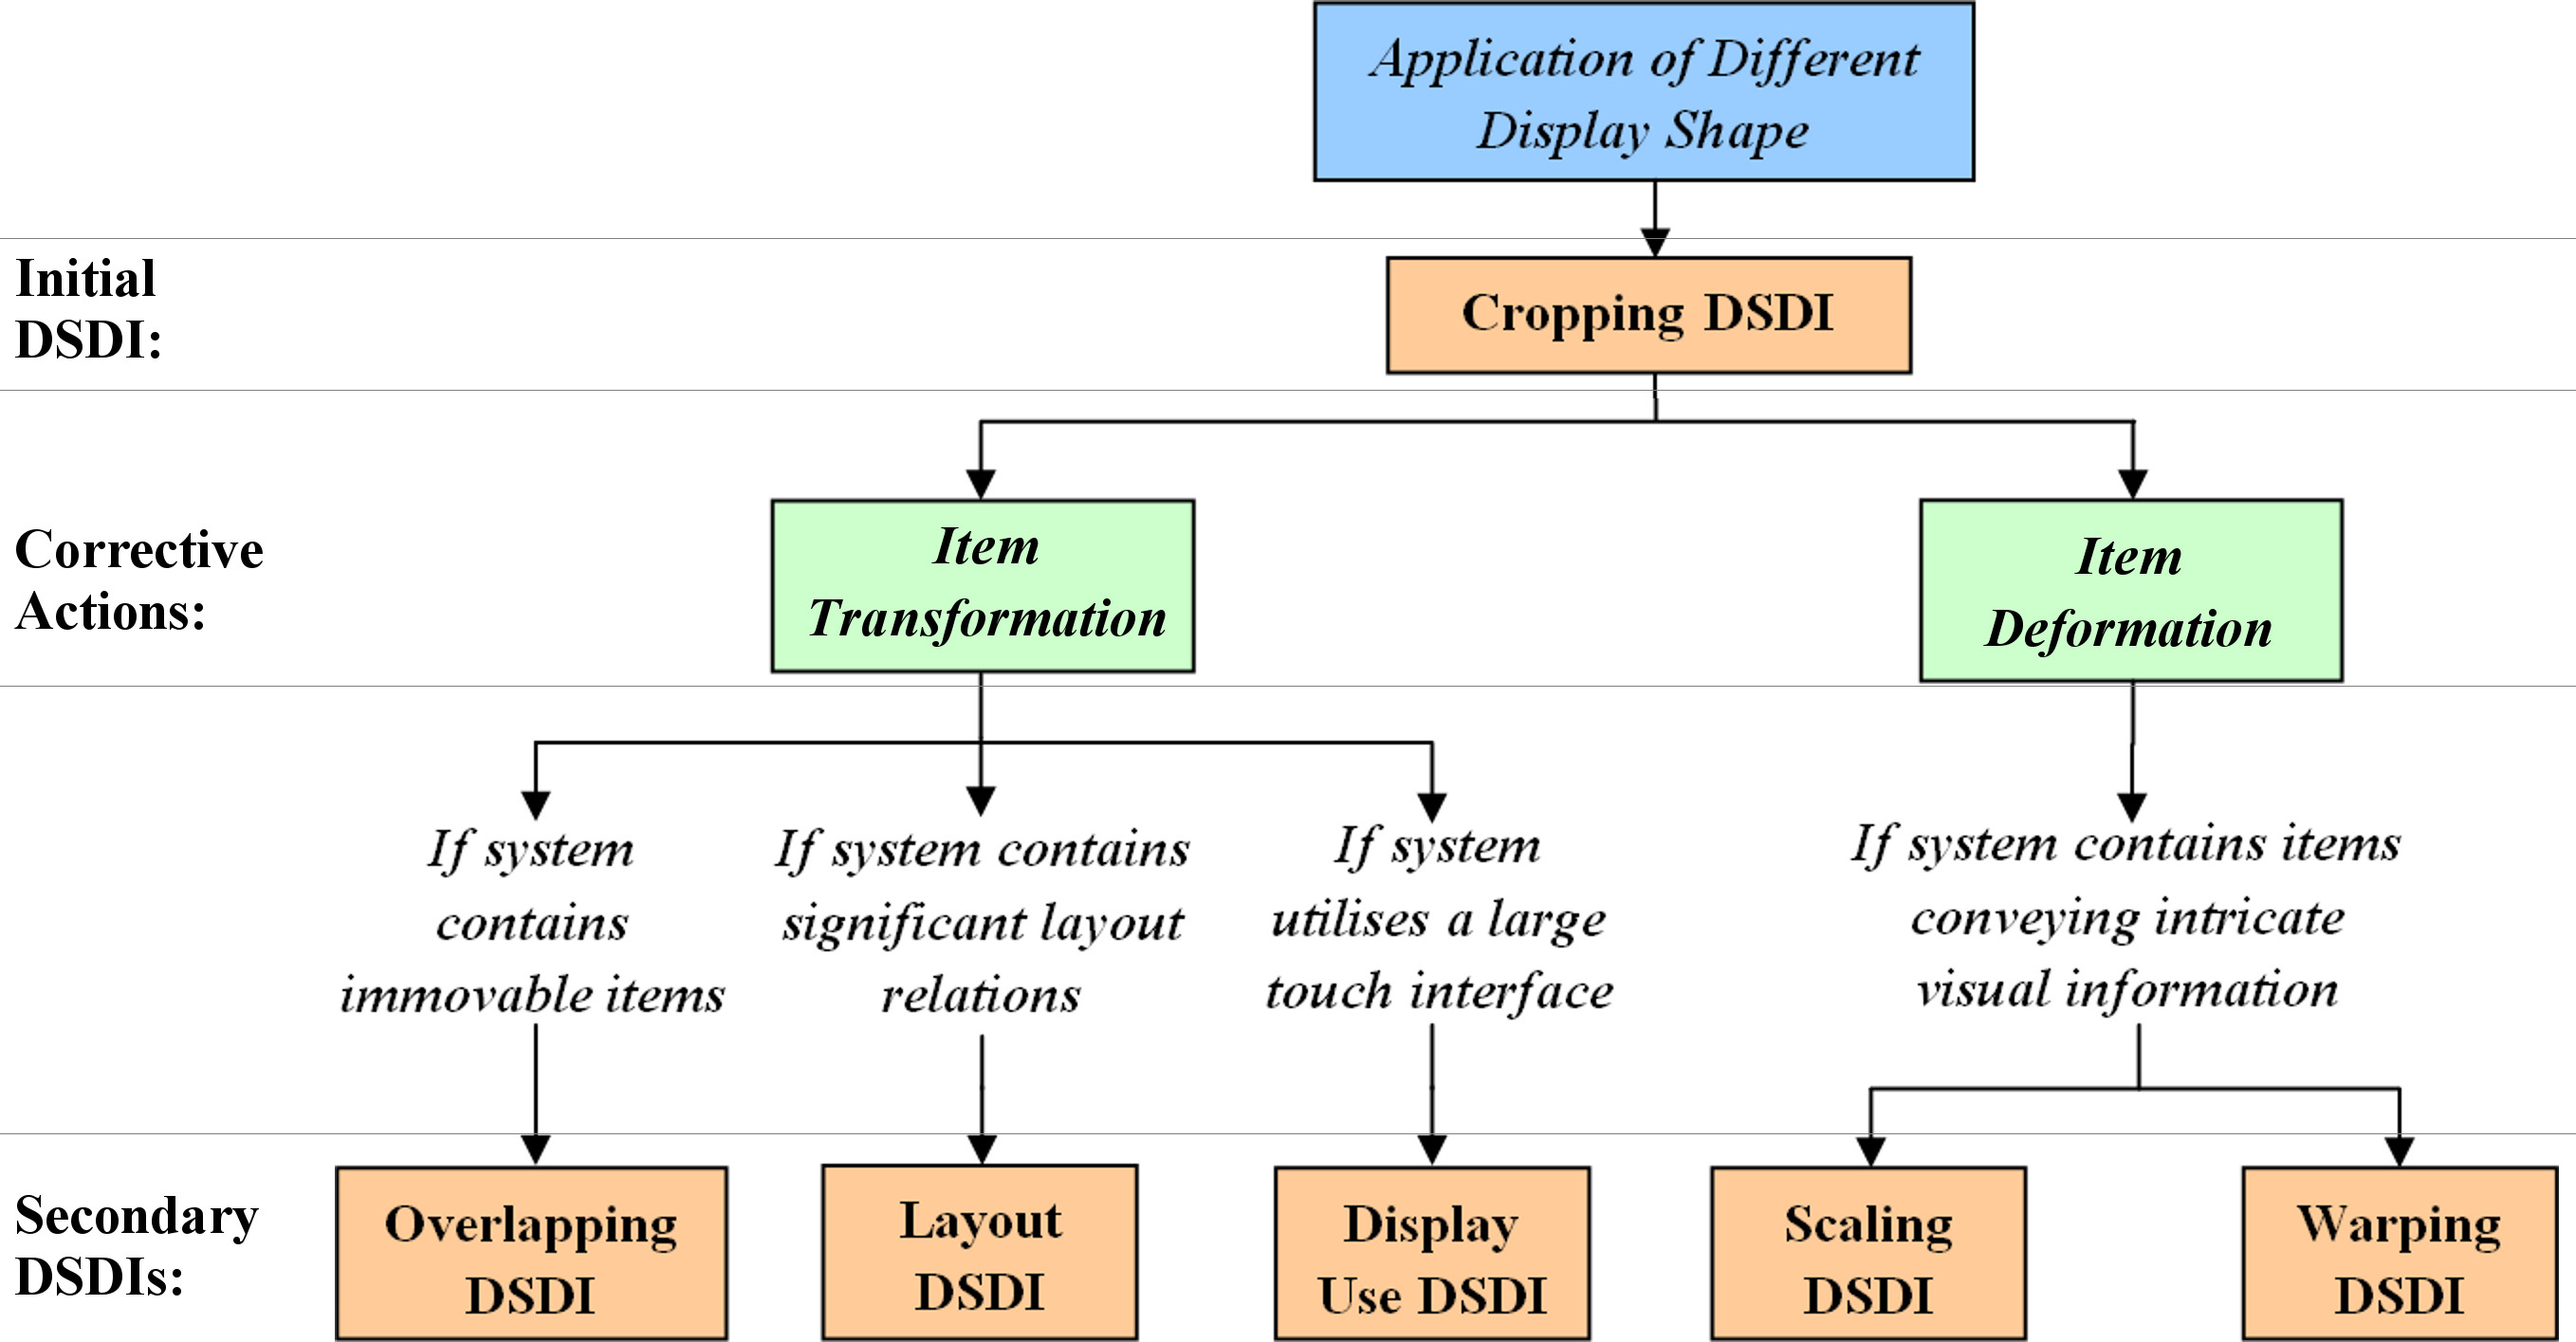
\includegraphics[width=0.95\textwidth]{figures/DSDIFlowChart.jpeg}
   \caption{A flow chat mapping the causality of Display Shape Dependence Issues (DSDIs).}
   \label{fig:dsdiFlow}
\end{figure*}

\begin{quote}\emph{i) \textbf{Cropping \ac{DSDI}:} Content items appear cropped as regions of them become positioned outside the display area.}\end{quote}

The scope of \acp{DSDI} outlined in this work is limited to environments where there is no hardware-level attempt to fit the visual contents to the display shape.
This is in keeping with the Section~\ref{sec:related} where the majority of works detailed create non-rectangular displays through showing a region of a rectangular output utilising approaches like partially covering parts of a display or occluding areas of a projection.

Cropping can have an effect of making the visual content items unfit for purpose; this is because the visual information they convey is lost.
Users may also be unable to interact directly with cropped items.
The cropping of visual content items outside the display area was also noted by Waldner et al. \cite{Waldner2011}.
Therefore, methods of resolving this cropping would be required to make software capable of adapting to different display shapes.
Attempts to resolve this cropping can result in secondary \acp{DSDI}.

\begin{quote}\emph{ii) \textbf{Overlapping \ac{DSDI}:} Occlusion from other visual content items.}\end{quote}

Attempts to resolve the {\emph{Cropping \ac{DSDI}}} can result in further issues such as the movement of content items, which did not previously overlap, to locations where they cover each other.
This overlapping of content items can result in regions of the visual content item becoming obscured.
This has the same negative impact as the {\emph{Cropping \ac{DSDI}}}.
Overlapping content items is not always an issue since the obscuring items could be moved by the user, but in systems where these items are immovable the occlusion would be irreparable.

\begin{quote}\emph{iii) \textbf{Layout \ac{DSDI}:} The loss of layout relations between visual content items.}\end{quote}

The changing of content item positions could be an issue in applications where layout is important; this is because the positioning of content items can imply their functional relations to the user~\cite{Constantine1999,mcnaughton-et-al:hcis2017}.
For example, controls in an application may be placed next to the items they influence.
If this layout relation is lost then it may confuse users what items the set of controls will influence. 
The loss of layout may not make content unfit for purpose but could be highly undesirable for software where the layout is intended to aid the user.
However, loss of layout is not always considered an issue meaning this \ac{DSDI} will only apply to specific content, tasks or applications.

\begin{quote}\emph{iv) \textbf{Scaling \ac{DSDI}:} The scaling of visual content items to an extreme.}\end{quote}

Scaling -- when a content item is resized whilst maintaining its aspect ratio -- of a visual element may be performed to avoid the cropping of content.
If this scaling is performed to an excessive degree, the visual information displayed by a content item may become incommunicable.
For example, if a content item displaying text is excessively scaled down, the characters it displays may become too small and be illegible to users.

\begin{quote}\emph{v) \textbf{Warping \ac{DSDI}:} The warping of visual content items.}\end{quote}

Warping is where the contents of a system are stretched and/or squashed in a non-uniform manner~\cite{Milliron2002}.
This could be applied to the entire visual output of a system to make it fit a particular display shape; however, this results in content items being stretched and squashed non-uniformly.
Even when the magnitude of this deformation is relatively small it can make any visual information a content item displays incommunicable to the user.
This \ac{DSDI} may not apply in all circumstances; some visual content items may display visual information which is communicable to the user no matter how severely it is deformed.
For example, if a content item's visual information is its colour -- if the item can be seen then it is successfully communicating its visual information to the user.

\begin{quote}\emph{vi) \textbf{Display Use \ac{DSDI}:} Display regions unused by the layout of visual content items.}\end{quote}

As a result of attempting to resolve the initial cropping, visual content items can often be translated to the same regions of the display, leaving large areas of an interface unused.
While this may not make the software unfit for purpose, it is not desirable for large tabletop interfaces.
This is due to the fact that on larger interfaces some regions of the display may be beyond a user's reach.
If the display uses direct touch interaction, then items in these regions become isolated from the user's influence.
There are solutions to this problem, such as users changing their positions around the interface or controls which can be used to indirectly manipulate out of reach items~\cite{Ryall2006a}.
However, if all the content items are constrained to a single region of the display beyond a user's reach, the need to repeatedly use these solutions is undesirable.
Changing positions to access remote content may not be possible in some environments due to the placement of the interface, for example, multi-touch interfaces may have several users positioned around them.
Users interacting simultaneously with a single interface often have a tendency to establish ``territories''~\cite{scott2004}.
A user wishing to move with these types of interfaces may disrupt others interacting with the system.
Solutions involving the remote control of out of reach content items result in users manipulating content items through a proxy~\cite{Smith11}.
This means that their interaction would no longer be direct, which can be undesirable because it counteracts the benefits of direct touch interaction~\cite{Schoning2008}.
Ensuring content items are capable of being spread out across the interface when possible reduces the likelihood that all the items will be placed beyond the reach of the users.\\

For a tabletop software system to be capable of dynamically adapting its visual content to different display shapes, the {\emph{Cropping \ac{DSDI}}} needs to be resolved in such a manner that will minimise the influence of any of the potential secondary \acp{DSDI}.
Figure~\ref{fig:dsdiFlow} maps the causality of the \acp{DSDI} and notes the circumstances in which they may have undesirable consequences on a system's visual content.
In the next section, using this list of \acp{DSDI}, we present a technique to adapt software to different display shapes in such a way that reduces the possibility of software becoming unusable due to these issues has been developed.

%-------------------------------------------------------------------------
\section{Minimising Display Shape Dependence Issues}
\label{sec:solution}

A novel technique was developed that would resolve the {\emph{Cropping \ac{DSDI}}} and would minimise the effect of any secondary \acp{DSDI}.
This technique is a method of adapting visual content items dynamically to different display shapes and comprises of two stages.
The first stage of the technique is built on the concept of taking the original visual output of the software and transforming it to fit within the borders of a new display shape.
This stage is referred to as {\em Virtual Projection}.
The second stage of the technique uses the difference between the shape of virtual projection and the display shape to ensure that the layout can, if needed, utilise all regions of the display.
This stage is referred to as {\em Position Pulling}.

\subsection{Virtual Projection}
\label{subsec:virtualprojection}

\begin{figure}[h!]
 \centering
   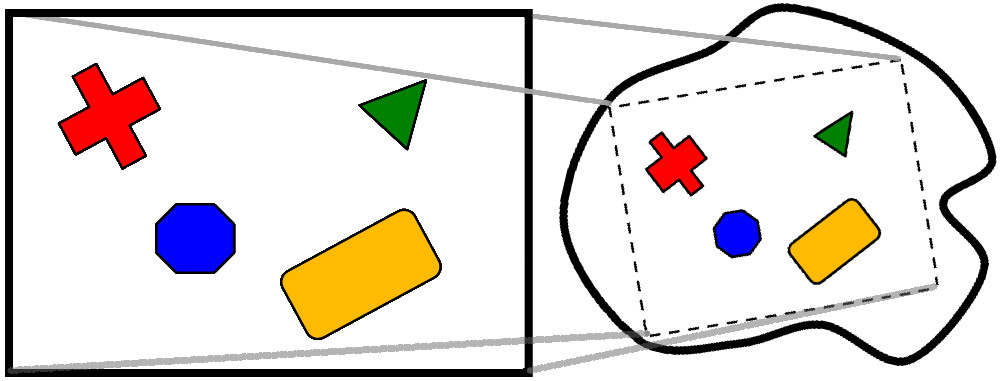
\includegraphics[width=0.45\textwidth]{figures/VirtualProjection.jpeg}
   \caption{An example of the {\emph{Virtual Projection}} stage.}
   \label{fig:virtualRectangle}
\end{figure}

For the first stage of the technique, the original shape of the software environment's visual output is treated as a single item.
This item, referred to as the virtual projection, is translated, rotated and scaled so that it fits within the display shape being used.
The transformations applied to the virtual projection are applied to any visual content items displayed in the software's original layout.

This stage of the technique has the effect of keeping the visual content items aligned with the virtual projection.
This ensures that visual contents will not incur occlusion from lying outside the borders of the new display shape, as the content items will all be contained within the virtual environment which fits inside the display.
Figure~\ref{fig:virtualRectangle} demonstrates how the virtual projection and its contents are transformed together to fit a new display shape.

As the original visual output of most current software is likely to be rectangular, the virtual projection for most systems can assumed to be a rectangle.
Finding the largest rectangle which can be placed within the display is required for this technique to utilise as much of the display as possible.
The concept of finding the largest rectangle inside a shape is a known as the {\emph{largest empty rectangle problem}} or the {\emph{maximal rectangle problem}}; there are several existing solutions to finding the maximal rectangle which can be utilised~\cite{Aggarwal1987,Naamad1984}.

Methods also exist for finding the largest of any specific polygon in the display shape~\cite{Toussaint1983}.
This allows for the adaptation of any software environment which may not have originally been rectangular.
Therefore the technique can be used to adapt software originally designed for any specific display shape to other display shapes.
As all the content items are translated, rotated and scaled by the same values their layout relations are preserved preventing the {\emph{Overlapping \ac{DSDI}}}.
As no warping deformations are used in this technique, there can be no occurrence of the {\emph{Warping \ac{DSDI}}}.
It is important to note that because of the scope of this work is limited to tabletop displays, the rotation of the content is not considered an issue.
By definition, tabletop interfaces are horizontal, allowing them to be accessed from any direction making the impact of orientation negligible.

However, there is the potential for issues with the {\emph{Scaling \ac{DSDI}}}; if the virtual projection is significantly smaller than the initial
layout's environment, then the contained content items will be scaled to an extreme value.
Indeed, it is possible that the content items may be scaled to an extent that they become unfit for purpose.
To counter this, the virtual projection technique adheres to scaling limits.
For systems where content items cannot be scaled to extremes, its content items should only be scaled to a predetermined limit.
This may result in sections of the content items becoming occluded from overlapping each other or from the display edge because they cannot be made small enough.
Without scale limits, the {\emph{Cropping}} and {\emph{Overlapping \acp{DSDI}}} are guaranteed not to occur but the {\emph{Scaling \ac{DSDI}}} remains a risk; with scale limits, the potential risk of \acp{DSDI} are reversed.
When utilising this technique, developers must decide on \ac{DSDI} trade-offs in their software.

This stage of the technique is similar to previously presented methods of dynamically adapting content to different displays which entails constricting the placement of content to a specific region of the displays used~\cite{Cotting2006,Raskar2003}.
This region is recreated for every display shape using the same dimensions, ensuring the contained content is kept relative to the region in layout, scale and orientation.

This stage of the technique does have the potential to minimise the effects of most of the \acp{DSDI}.
However, this stage of the technique does not counter the occurrence of the {\emph{Display Use \ac{DSDI}}} since only a single region of the display, the virtual projection, is used.

\subsection{Position Pulling}
\label{subsec:positionpulling} 

\begin{figure}[h!] 
 \centering
   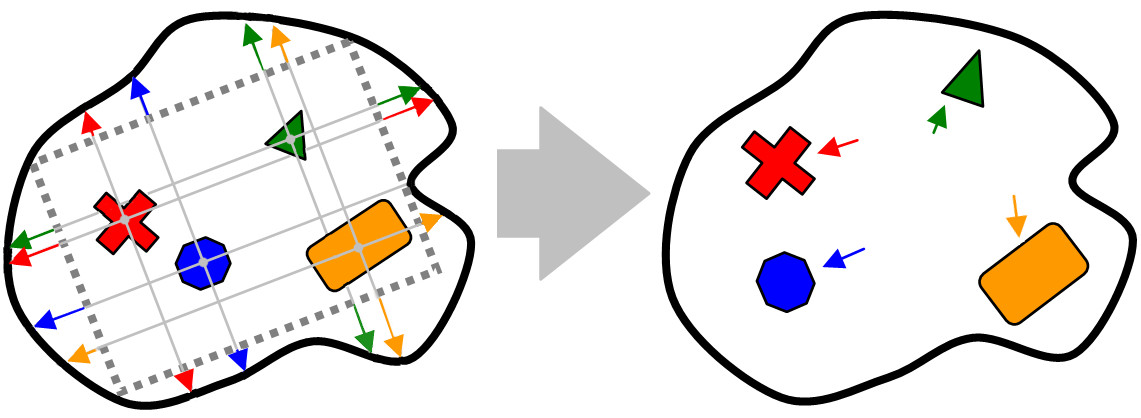
\includegraphics[width=0.45\textwidth]{figures/PositionPulling.jpeg}
   \caption{An example of the {\emph{Position Pulling}} stage.}
   \label{fig:pullLayout}
\end{figure}

For the second stage of the technique, the gaps between the virtual projection and the display edges are utilised.
The objective of this stage is to move content items into areas of the display which are left unused by the virtual projection.
The edges of the virtual projection exert a \lq pulling force\rq\ on content items.
The magnitude of this force is determined by the size of gaps between the display border and the virtual projection edges.
The magnitudes of these \lq pulling forces\rq\ are also influenced by a content item's proximity to the edge instigating the force.
Content items are pulled from their centroids to keep calculations simple; this means the shapes and sizes of the items moved are ignored.

The position pulling stage results in pulling content items into unused regions of the display (see
Figure~\ref{fig:pullLayout}).
Items positioned near large gaps between the virtual projection and the display borders are pulled into these areas.
The left hand side of Figure~\ref{fig:pullLayout} shows the \lq pulling forces\rq\ which result from the gaps between the virtual projection area edges adjacent to the content items.
Figure~\ref{fig:pullLayout}'s right hand side shows the translation of the content items resulting from the combined influence of the \lq pulling forces\rq .

\begin{figure}[h!]
 \centering
   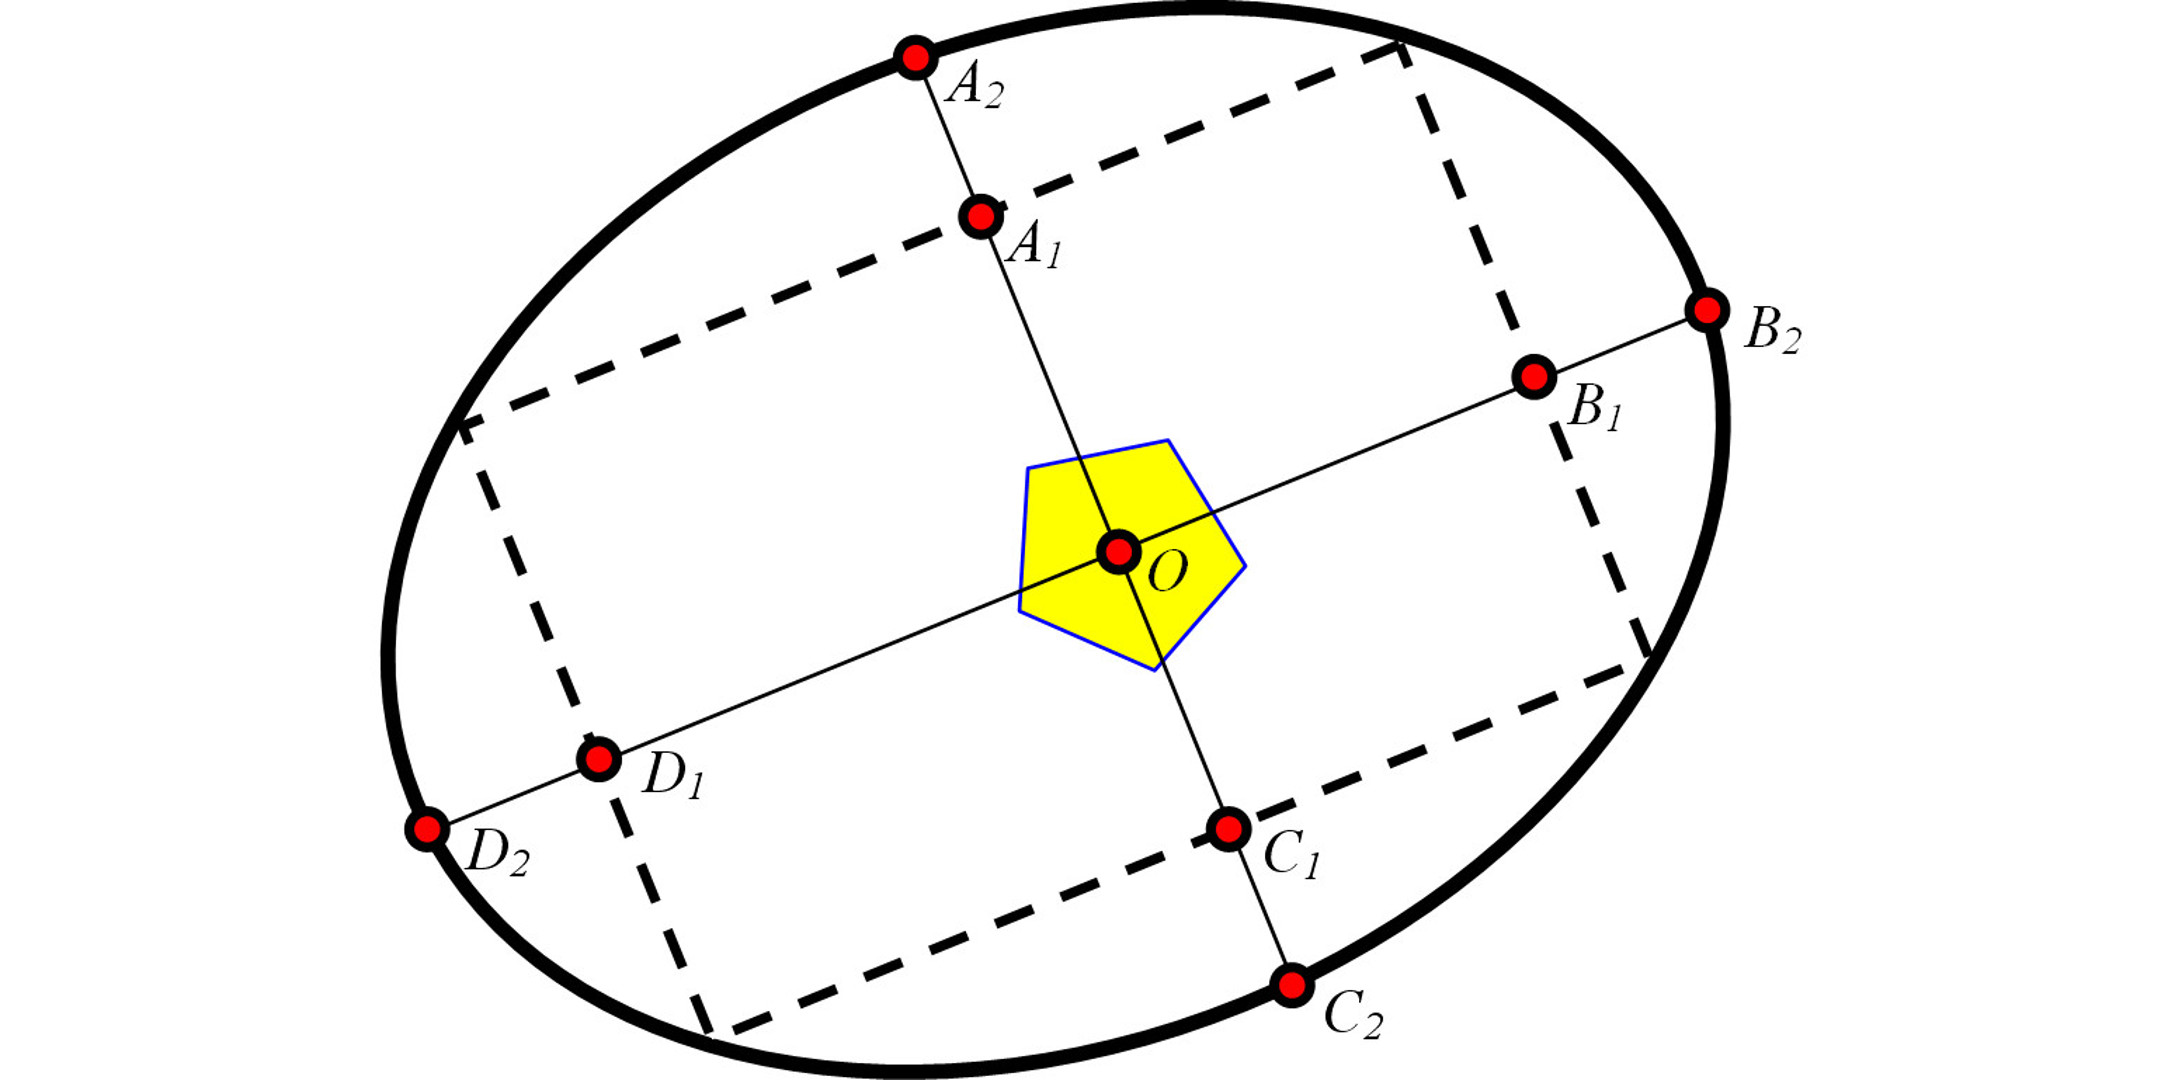
\includegraphics[width=0.45\textwidth]{figures/DetailedPositionPulling.jpeg}
   \caption{Detailed view of the information used in {\emph{Position Pulling}}.}
   \label{fig:pullLayoutExp}
\end{figure}

\section*{Algorithms}

\begin{algorithm}[h!]
\caption{Calculating the \lq pulling force\rq~vectors.}
\label{algo:pullLayoutOne}
\begin{algorithmic}
\STATE \textbf{getPullVectors}($O,\ A_{1},\ A_{2},\ B_{1},\ B_{2},\ C_{1},\ C_{2},\ D_{1},\ D_{2}$)
\INDSTATE[2]$\overrightarrow{LEFT}\hspace{0.5cm} \leftarrow \hspace{0.25cm}(\overrightarrow{D_{1}D_{2}}\ *\ ( |\overrightarrow{OD_{1}}|\  /\ |\overrightarrow{B_{1}D_{1}}| )$
\INDSTATE[2]$\overrightarrow{RIGHT}\hspace{0.25cm} \leftarrow \hspace{0.25cm}(\overrightarrow{B_{1}B_{2}}\ *\ ( |\overrightarrow{OB_{1}}|\  /\ |\overrightarrow{B_{1}D_{1}}| )$
\INDSTATE[2]$\overrightarrow{UP}\hspace{1cm} \leftarrow \hspace{0.25cm}(\overrightarrow{A_{1}A_{2}}\ *\ ( |\overrightarrow{OC_{1}}|\  /\ |\overrightarrow{A_{1}C_{1}}| )$
\INDSTATE[2]$\overrightarrow{DOWN}\hspace{0.3cm} \leftarrow \hspace{0.25cm}(\overrightarrow{C_{1}C_{2}}\ *\ ( |\overrightarrow{OA_{1}}|\  /\ |\overrightarrow{A_{1}C_{1}}| )$
\STATE \textit{return}\ $\overrightarrow{LEFT},\ \overrightarrow{RIGHT},\ \overrightarrow{UP},\ \overrightarrow{DOWN}$
\end{algorithmic}
\end{algorithm}

\begin{algorithm}[h!]
\caption{Applying the \lq pulling force\rq~vectors.}
\label{algo:pullLayoutTwo}
\begin{algorithmic}
\STATE \textbf{applyPull}($item,\ \theta,\ \overrightarrow{LEFT},\ \overrightarrow{RIGHT},\ \overrightarrow{UP},\ \overrightarrow{DOWN}$)
\INDSTATE[2]$\overrightarrow{PULL} \leftarrow \overrightarrow{LEFT} + \overrightarrow{RIGHT} + \overrightarrow{UP} + \overrightarrow{DOWN}$
\INDSTATE[2]$\overrightarrow{PULL}.rotateBy(\theta)$
\INDSTATE[2]$item.translateBy(\overrightarrow{PULL})$
\STATE \textit{return}
\end{algorithmic}
\end{algorithm}

Algorithm~\ref{algo:pullLayoutOne} shows how each vector representing the individual \lq pulling force\rq\ is calculated and made proportional to the item's proximity to the corresponding edge.
Algorithm~\ref{algo:pullLayoutTwo} details how pulling force vectors are attained, where $\theta$ represents the orientation of the virtual projection.
The existing values used in Algorithm~\ref{algo:pullLayoutOne} and Algorithm~\ref{algo:pullLayoutTwo} correspond to those presented in Figure~\ref{fig:pullLayoutExp}.

This stage of the technique effectively deforms the layout of the content items by warping it to fit the display shape.
Though the layout is warped, the content items are not deformed in any way by this stage of the technique.
The deformation of the layout ensures that more of the display's real estate is utilised and that the layout is not constrained to a small region of the display.
This minimises the potential effects of the {\emph{Display Use \ac{DSDI}}}.
The shape of the item does not influence the pull vectors, only the point it uses for translation.
Taking the shape into account would require significantly more processing and would only result in a marginally more accurate pull vector.

The \lq pulling forces\rq\ used in this stage of the technique assume the original environment of a piece of software is rectangular.
Assuming a rectangular environment can be considered acceptable due to the current prevalence of software intended for use with rectangular displays~\cite{VanDam2001}.
However, it is possible that in the future the technique may need to adapt software designed for non-rectangular displays to different shapes.
The virtual projection stage can easily adapt to this through using the maximal polygon opposed to the maximal rectangle.
For the position pulling stage to utilise content intended for a non-rectangular display, a vector representing the \lq pulling force\rq\ for every unique edge of the virtual projection would need to be created.
Vector addition between each of these vectors representing the \lq pulling forces\rq\ then creates a single vector which can be used to translate a content item.

\subsection{Technique Observations}
\label{subsec:techniqueobservations} 

After employing the two stages discussed, the resulting technique has the potential to minimise any of the \acp{DSDI} identified. 
Due to the development of this technique for use on tabletop displays it is limited to use on two-dimensional displays which are positioned horizontally.
The technique allows for interventions at different points which can depend on how content should be treated, giving developers greater control over the influence and impact of the technique.
This, in addition to the fact that the technique uses only linear transformations resulting in a simple to implement piece of functionality, makes the presented technique a promising approach to handling different display shapes on tabletops in real-world applications.


%-------------------------------------------------------------------------
\section{Study}
\label{sec:study}

A study was carried out where an implementation of the technique discussed  in the previous section was tried on several different software applications with several different display shapes.

\subsection{Implementation of the Technique}
\label{subsec:implementation} 

The technique was implemented into version 2.1 of the {\emph{SynergyNet}} framework~\cite{McNaughton2017,AlAgha2010}, a multi-touch software framework intended for use with rectangular tabletop interfaces.
The framework functions by rendering a range of content items, such as images, text and video, which can then be manipulated by users.
{\emph{SynergyNet}} is built in Java, allowing it to be run across different operating systems and can accept a wide range of different multi-touch protocols such as TUIO~\cite{Kaltenbrunner2007}.
The framework's ability to adapt to different systems makes it a suitable candidate for use with different display shapes.

\begin{figure*}[h!] 
 \centering
   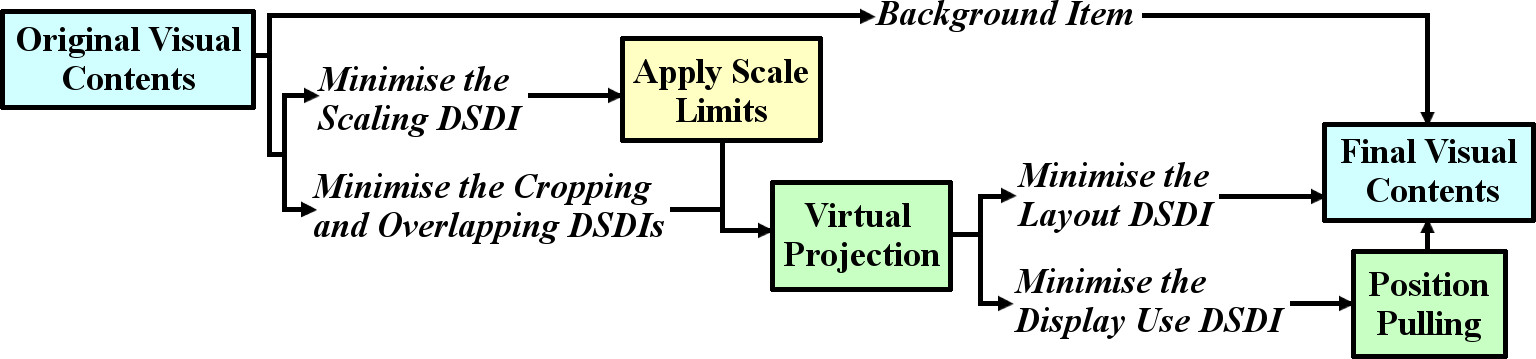
\includegraphics[width=0.95\textwidth]{figures/TechniqueFlowchart.jpeg}
   \caption{Flowchart demonstrating navigation of the technique.}
   \label{fig:flowchart}
\end{figure*}

Another reason for the choice of the {\emph{SynergyNet}} framework was the range of applications written using it which are readily available.
The technique was implemented into the framework which allowed any application written for this version of {\emph{SynergyNet}} to potentially utilise different display shapes.
The available applications are produced by a number of different developers for different purposes, allowing for the technique to be tried with a range of contents with not just differing layouts, but also differing significance to their layouts.

For the technique to work the software needs to be informed of the dimensions of the display shape currently available.
This is done through the creation of files containing vectors which corresponding to a display shape which the framework can utilise.
These vector files also include information on the display shape's maximal polygon (a rectangle is used as all previous {\emph{SynergyNet}} applications were built assuming a rectangular display).

Figure~\ref{fig:flowchart} shows the options available to applications developers utilising the technique.
Choices made in its usage, such as which stages of the technique are employed and the constraints placed on these stages, can influence which \acp{DSDI} it prevents and counters.
For example, if a developer wishes a content item to act as the background to the entire display, and its cropping is not an issue, then both stages of the technique can be circumvented.
For content items not set aside to be background images, developers can choose whether or not to apply the position pulling stage of the technique.
If applied, the content items will maximise the use of the display shape's real estate by being pulled into previously unused areas of the display.
However, if the layout of the content items is of a greater importance than the maximisation of display usage, the developer can choose to disregard the position pulling stage for any content items in the layout.


\subsection{Selection of Applications}
\label{subsec:selectionofapplications} 

The implemented technique was tested using a number of applications created by several developers for previous studies in the {\emph{SynergyNet}} project~\cite{higgins2011}.
The study focused on two specific applications, {\emph{Grid}} and {\emph{Simple Map} (see Figure~\ref{fig:apps}):\\

\begin{itemize}
  \item {\emph{\textbf{Grid}}}: 
  Nine items are positioned in a grid layout which users can reposition, rotate and scale through multi-touch gestures.
  This is one of the applications supported by the {\emph{SynergyNet}} framework which help familiarise users to interacting with a large multi-touch interface. 
    \begin{itemize}
    \item  All the content in this application is specifically positioned.
    \item The locational relation between all the items in this application is very significant.
  \end{itemize}
    \item {\emph{\textbf{Simple Map}}}: 
  Users supply countries in a configuration file and the application will show a world map when started with the specified countries' flags positioned on top of them; users can then move the flag items around the map.
    \begin{itemize}
    \item  All the content in this application is specifically positioned.
    \item The locational relation between the flag items and the background image is strong.
  \end{itemize}
\end{itemize}

These two were chosen because of the varying significance of their items' layout.
This was important because the study intended to investigate how the technique would impact on the arrangement of items with a significant layout.

\begin{figure}[h!] 
 \centering
  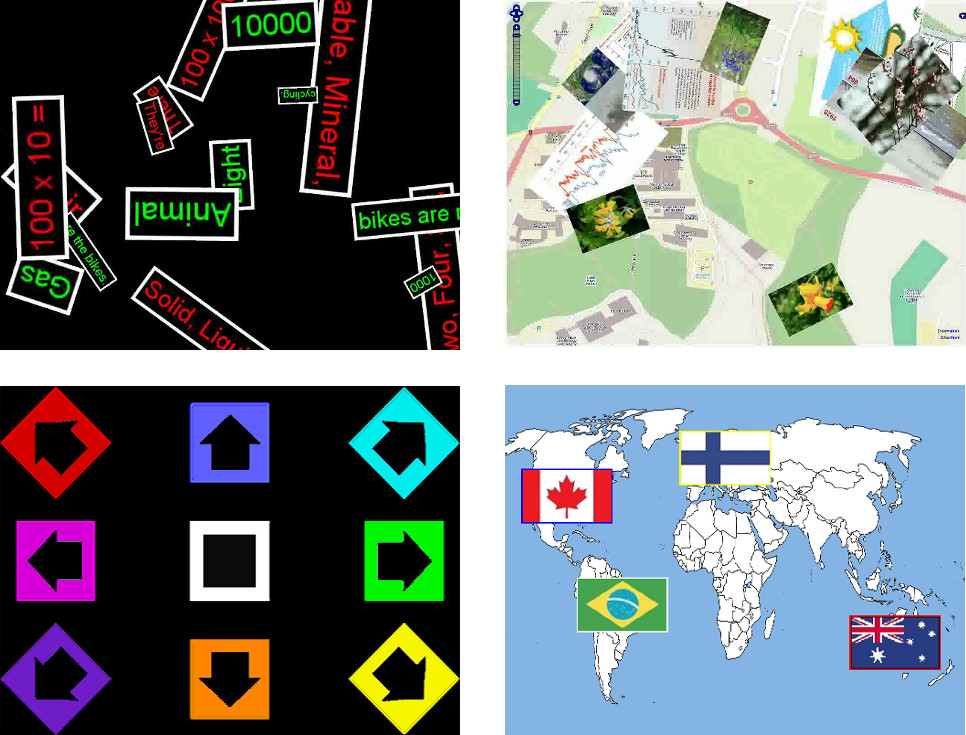
\includegraphics[width=0.45\textwidth]{figures/Applications.jpeg}
  \caption{The applications chosen for observation, from left to right:  {\emph{Grid}} and {\emph{Simple Map}}.}
  \label{fig:apps}
\end{figure}


\subsection{Selection of Display shapes}
\label{subsec:selectionofdisplayshapes} 

\begin{figure*}[h!] 
 \centering
  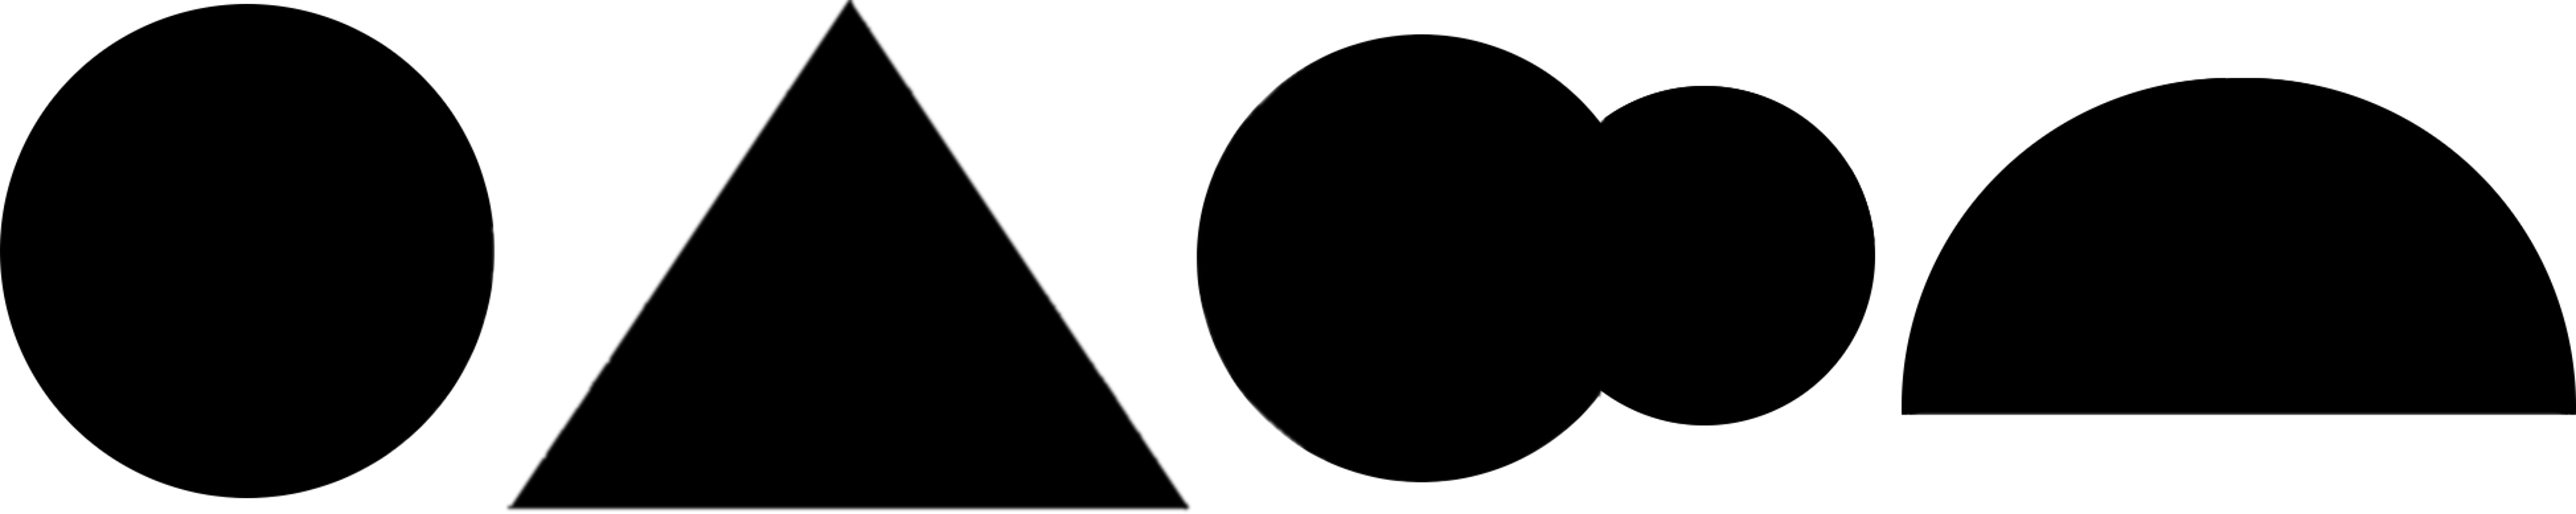
\includegraphics[width=0.95\textwidth]{figures/DisplayShapes.jpeg}
  \caption{The display shapes chosen for observation, from left to right:  {\emph{Circle}}, {\emph{Triangle}}, {\emph{Intersecting Circles}} and {\emph{Semi-circle}}.}
  \label{fig:displayshapes}
\end{figure*}

The {\emph{SynergyNet}} framework was adapted to assume the use of a range of display shapes.
These shapes were chosen after consultation with a furniture manufacturer who had experience with designing multi-touch tables.
The manufacturer was in a strong industry position for making predictions concerning the likely design features of future multi-touch tabletops, including their display shapes; the shapes chosen are shown in Figure~\ref{fig:displayshapes}.

Some of these shapes were derived from common table shapes which could be used with tabletop interfaces, such as the semi-circle design.
This allows for users positioned around the display in various places to have an equal share of the interface which can be beneficial to collaboration.
The circle shape was also chosen for its ability to allow users to have equal shares of the display.
The triangle was chosen because of its regular nature, meaning that all its sides and corners are congruent.
The intersecting circles shape was designed to make further use of multi-touch's facilitation of collaboration by providing focal points and areas to share content items in.
The larger circle of the display shape can be used for one activity such as displaying content items whereas the smaller circle could be used for another activity such as manipulating the items.
The semi-circle was selected due to the common usage of the shape for tables.


\subsection{Approach}
\label{subsec:approach} 

In the study, both stages of the technique were set to always be applied to the content items to investigate the full impact of the technique.
No limitations were placed on the technique in the study either.
The technique was implemented in such a way that it was applied to the initial layout of content in an application.

The four different display shapes were emulated in the study by using a large rectangular display shape, then covering parts of the screen used to make the visible area of the shape match an intended display shape.
Both of the applications of the study were run with each of the four display shapes.
The framework was set up to capture screenshots taken at various points during the application of the technique; before applications, after the placement of the display shape's outline (blanking out anything that would not visible on the display),  after the virtual projection stage and after the position pulling stage.


\subsection{Data Analysis}
\label{subsec:dataanalysis} 

The impact of the technique on the \acp{DSDI} was planned to be measured using the screenshots taken during the execution of the technique.
For each combination of the two software applications and four display shapes, the presence of \acp{DSDI} can be ascertained.
For each \ac{DSDI} a measurement was outlined which could be obtained from the screenshots.
These measurements were then used to evaluate the impact of the various stages of the technique on the \acp{DSDI}.
The measurements have all been converted to percentages to allow for simple comparison between the applications, as the size of the layouts, initial scales and number of items will differ.
These measurements were as follows:
\begin{itemize}
  \item \textbf{Occluded Items}: 
  To measure impact on the Cropping \ac{DSDI} the number of items suffering occlusion from the display shape expressed as a percentage is used.
  \item \textbf{Overlapping Items}: 
  To measure impact on the Overlapping \ac{DSDI} the number of items suffering occlusion from other items is used.  
  \item \textbf{Change in Layout}: 
  To measure impact on the Layout \ac{DSDI} the distance of items from where they were expected to be with a layout of the same scale and orientation (but no other deformations) is measured.
  This average of these value, expressed as a percentage of the width of the layout's minimal bounding rectangle is used.
  \item \textbf{Display Shape Unused}: 
  To measure impact on the Display Use \ac{DSDI} a minimal bounding rectangle is drawn around the visual content.
  The area unused (i.e. are of the display outside the rectangle) divided by the total area of the display shape gives the area that goes unused as a percentage.
  \item \textbf{Change in Scale}: 
  To measure impact on the Scaling \ac{DSDI} the absolute maximum change in scale of all the item in the app expressed as a percentage of the item's original scale is used.
  \item \textbf{Deformed Items}: 
  To measure impact on the Scaling \ac{DSDI}  the number of items being deformed in a non-uniform manner expressed as a percentage is used.
\end{itemize}


%-------------------------------------------------------------------------
\section{Results}
\label{sec:results}

The results are summarised for each application per shape and phase in Tables \ref{tab:gridApp} and \ref{tab:mapApp}.
The phases used in the tables represent the following stages of the execution of the technique as follows:
\begin{itemize}
  \item \textbf{Phase 0}: 
  When the application is first started before the execution of the technique starts.
  \item \textbf{Phase 1}: 
  After the display shape borders are applied to the application.
  \item \textbf{Phase 2}: 
  After the virtual projection stage of the technique is carried out.
  \item \textbf{Phase 3}: 
  After the pull positions stage of the technique is completed.
\end{itemize}

\subsection{Grid Application}
\label{subsec:gridresults} 

\begin{table*}[p]
	\centering
	\begin{tabular}{ | l | c | c | c | c | c | c | c | }	
	\hline
	\multicolumn{8}{|c|}{\textbf{Grid Application}} \\
	\hline
	& & \multicolumn{6}{c|}{\textbf{\ac{DSDI} Measurements}} \\
	\cline{3-8}
		& & & & \textbf{Change} & & \textbf{Change} & \\
		& & \textbf{Occluded} & \textbf{Overlapping} & \textbf{in} & \textbf{Display Shape} & \textbf{in} & \textbf{Deformed} \\
		\textbf{Shape} & \textbf{Phase} & \textbf{Items} & \textbf{Items} & \textbf{Layout} & \textbf{Unused} & \textbf{Scale} & \textbf{Items} \\ 
	\hline
		Rectangle & 0 & 0\% & 0\% & 0\% & 0\% & 0\% & 0\% \\  
	\hline
		\multirow{3}{*}{Circle} & 1 & 66.7\% & 0\% & 0\% & 0\% & 0\% & 0\% \\ \smallline
		& 2 & 0\% & 0\% & 0\% & 35.8\% & 39.5\% & 0\% \\ \smallline
		& 3 & 0\% & 0\% & 6.4\% & 20.9\% & 39.5\% & 0\% \\
	\hline
		\multirow{3}{*}{Triangle} & 1 & 77.8\% & 0\% & 0\% & 0\% & 0\% & 0\% \\ \smallline
		& 2 & 0\% & 0\% & 0\% & 50.1\% & 48.8\% & 0\% \\ \smallline
		& 3 & 0\% & 0\% & 20.7\% & 7.6\% & 48.8\% & 0\% \\
	\hline
		\multirow{3}{*}{Intersecting Circles} & 1 & 66.7\% & 0\% & 0\% & 0\% & 0\% & 0\% \\ \smallline
		& 2 & 0\% & 0\% & 0\% & 56.9\% & 44.2\% & 0\% \\ \smallline
		& 3 & 0\% & 0\% & 27.4\% & 14.6\% & 44.2\% & 0\% \\
	\hline
		\multirow{3}{*}{Semi-circle} & 1 & 88.9\% & 0\% & 0\% & 0\% & 0\% & 0\% \\ \smallline
		& 2 & 0\% & 0\% & 0\% & 40.9\% & 44.2\% & 0\% \\ \smallline
		& 3 & 0\% & 0\% & 11.9\% & 13\% & 44.2\% & 0\% \\ 
	\hline
	\end{tabular}
	\caption{The \ac{DSDI} measurements from the study in {\emph{SynergyNet}}'s {\emph{Grid}} application.}
	\label{tab:gridApp}
\end{table*}

\begin{figure*}[p]
 \centering
  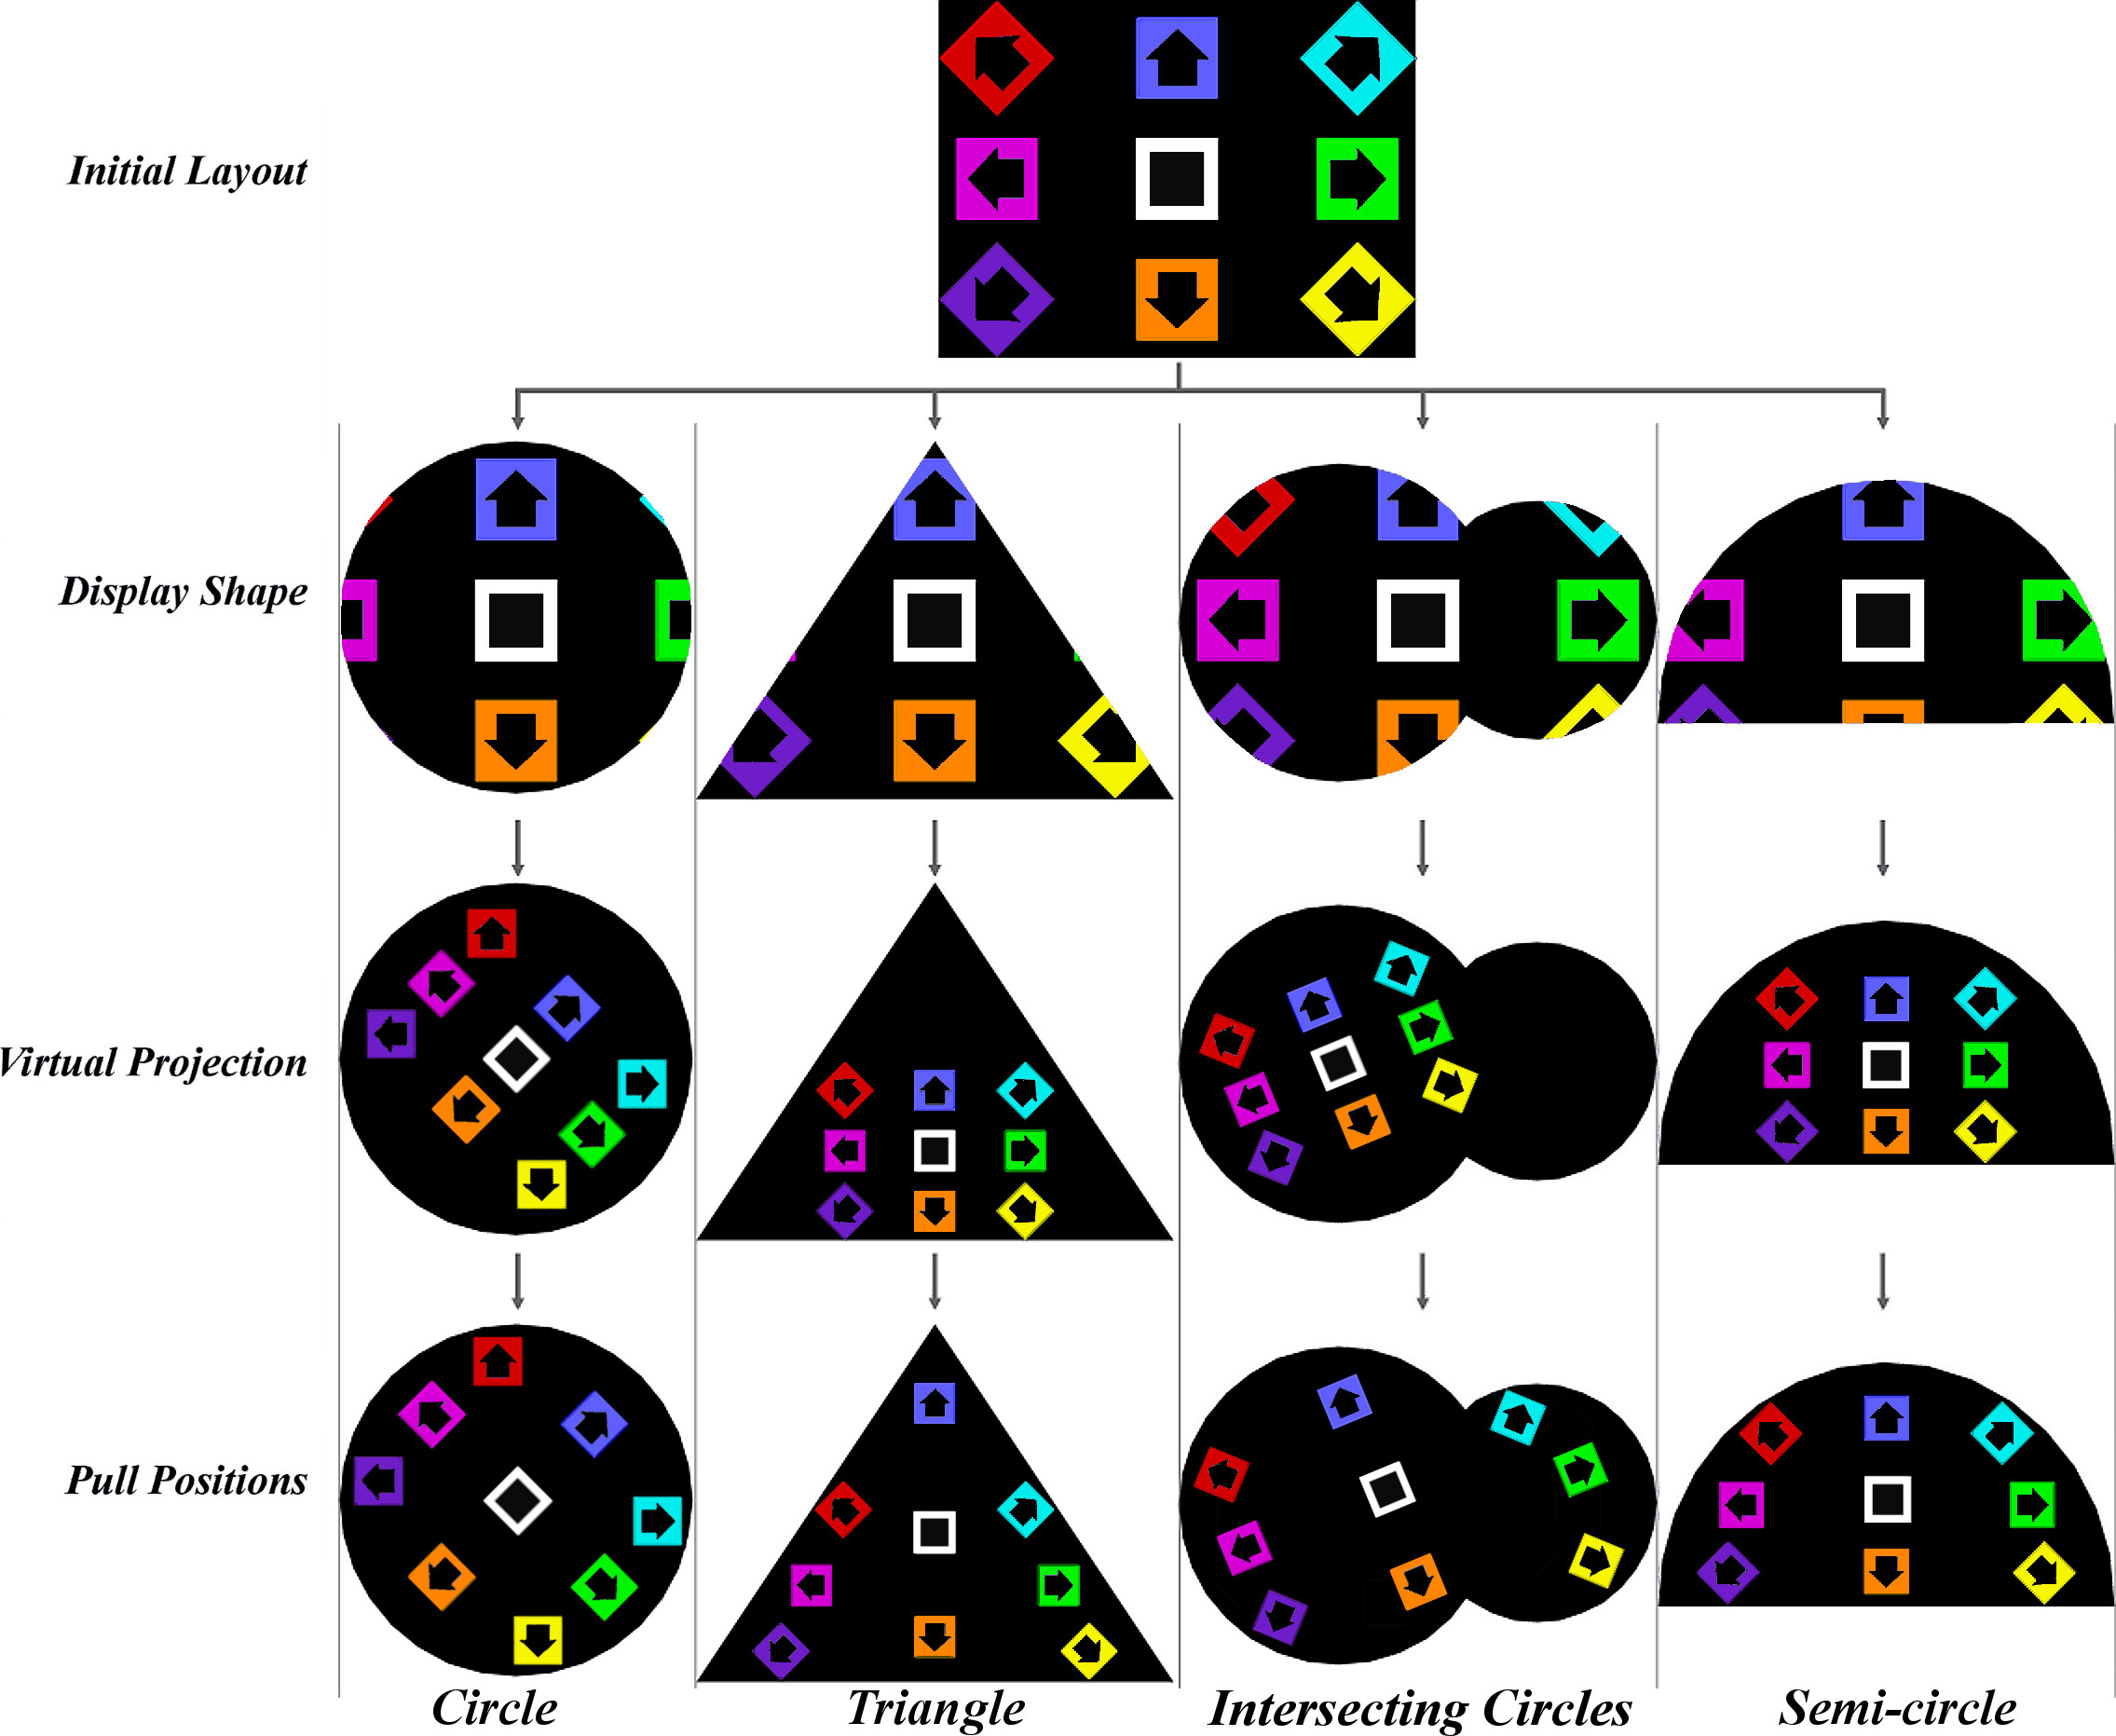
\includegraphics[width=0.9\textwidth]{figures/GridApplication.jpeg}
  \caption{Influence of the implemented technique on {\emph{SynergyNet}}'s {\emph{Grid}} application.}
  \label{fig:gridApp}
\end{figure*}

Table~\ref{tab:gridApp} shows that the technique reduced the initial occlusion for all shapes without incurring any occlusion from overlapping items or deformation of items throughout its execution.
However, the virtual projection stage did increase the change in scale and the amount of the display shape which went unused.
The pull positions stage of the technique did reduce the amount of the display shape which went unused quite significantly for some shapes but did increase the change in layout.
The change in layout for some of the display shapes was quite significant; for example, the triangle as shown in Figure~\ref{fig:gridApp} where the grid layout becomes nearly unrecognisable.


\subsection{Simple Map Application}
\label{subsec:simplemapresults} 

\begin{table*}[p]
	\begin{tabular}{ | l | c | c | c | c | c | c | c | }	
	\multicolumn{8}{c}{ } \\
	\hline
	\multicolumn{8}{|c|}{\textbf{Simple Map Application}} \\
	\hline
	& & \multicolumn{6}{c|}{\textbf{\ac{DSDI} Measurements}} \\
	\cline{3-8}
		& & & & \textbf{Change} & & \textbf{Change} & \\
		& & \textbf{Occluded} & \textbf{Overlapping} & \textbf{in} & \textbf{Display Shape} & \textbf{in} & \textbf{Deformed} \\
		\textbf{Shape} & \textbf{Phase} & \textbf{Items} & \textbf{Items} & \textbf{Layout} & \textbf{Unused} & \textbf{Scale} & \textbf{Items} \\ 
	\hline
		Rectangle & 0 & 0\% & 20\% & 0\% & 0\% & 0\% & 0\% \\  
	\hline
		\multirow{3}{*}{Circle} & 1 & 60\% & 20\% & 0\% & 0\% & 0\% & 0\% \\ \smallline
		& 2 & 0\% & 20\% & 0\% & 37.9\% & 42\% & 0\% \\ \smallline
		& 3 & 0\% & 20\% & 5.2\% & 37.1\% & 42\% & 0\% \\
	\hline
		\multirow{3}{*}{Triangle} & 1 & 100\% & 20\% & 0\% & 0\% & 0\% & 0\% \\ \smallline
		& 2 & 0\% & 20\% & 0\% & 50.2\% & 50\% & 0\% \\ \smallline
		& 3 & 0\% & 20\% & 17.6\% & 22.7\% & 50\% & 0\% \\
	\hline
		\multirow{3}{*}{Intersecting Circles} & 1 & 80\% & 20\% & 0\% & 0\% & 0\% & 0\% \\ \smallline
		& 2 & 0\% & 20\% & 0\% & 58.1\% & 48.2\% & 0\% \\ \smallline
		& 3 & 0\% & 20\% & 16.4\% & 42\% & 48.2\% & 0\% \\
	\hline
		\multirow{3}{*}{Semi-circle} & 1 & 80\% & 20\% & 0\% & 0\% & 0\% & 0\% \\ \smallline
		& 2 & 0\% & 20\% & 0\% & 40.3\% & 44.6\% & 0\% \\ \smallline
		& 3 & 0\% & 20\% & 9.9\% & 28.2\% & 44.6\% & 0\% \\ 
	\hline
	\end{tabular}
	\caption{The \ac{DSDI} measurements from the study in {\emph{SynergyNet}}'s {\emph{Simple Map}} application.}
	\label{tab:mapApp}
\end{table*}

\begin{figure*}[p]
 \centering
  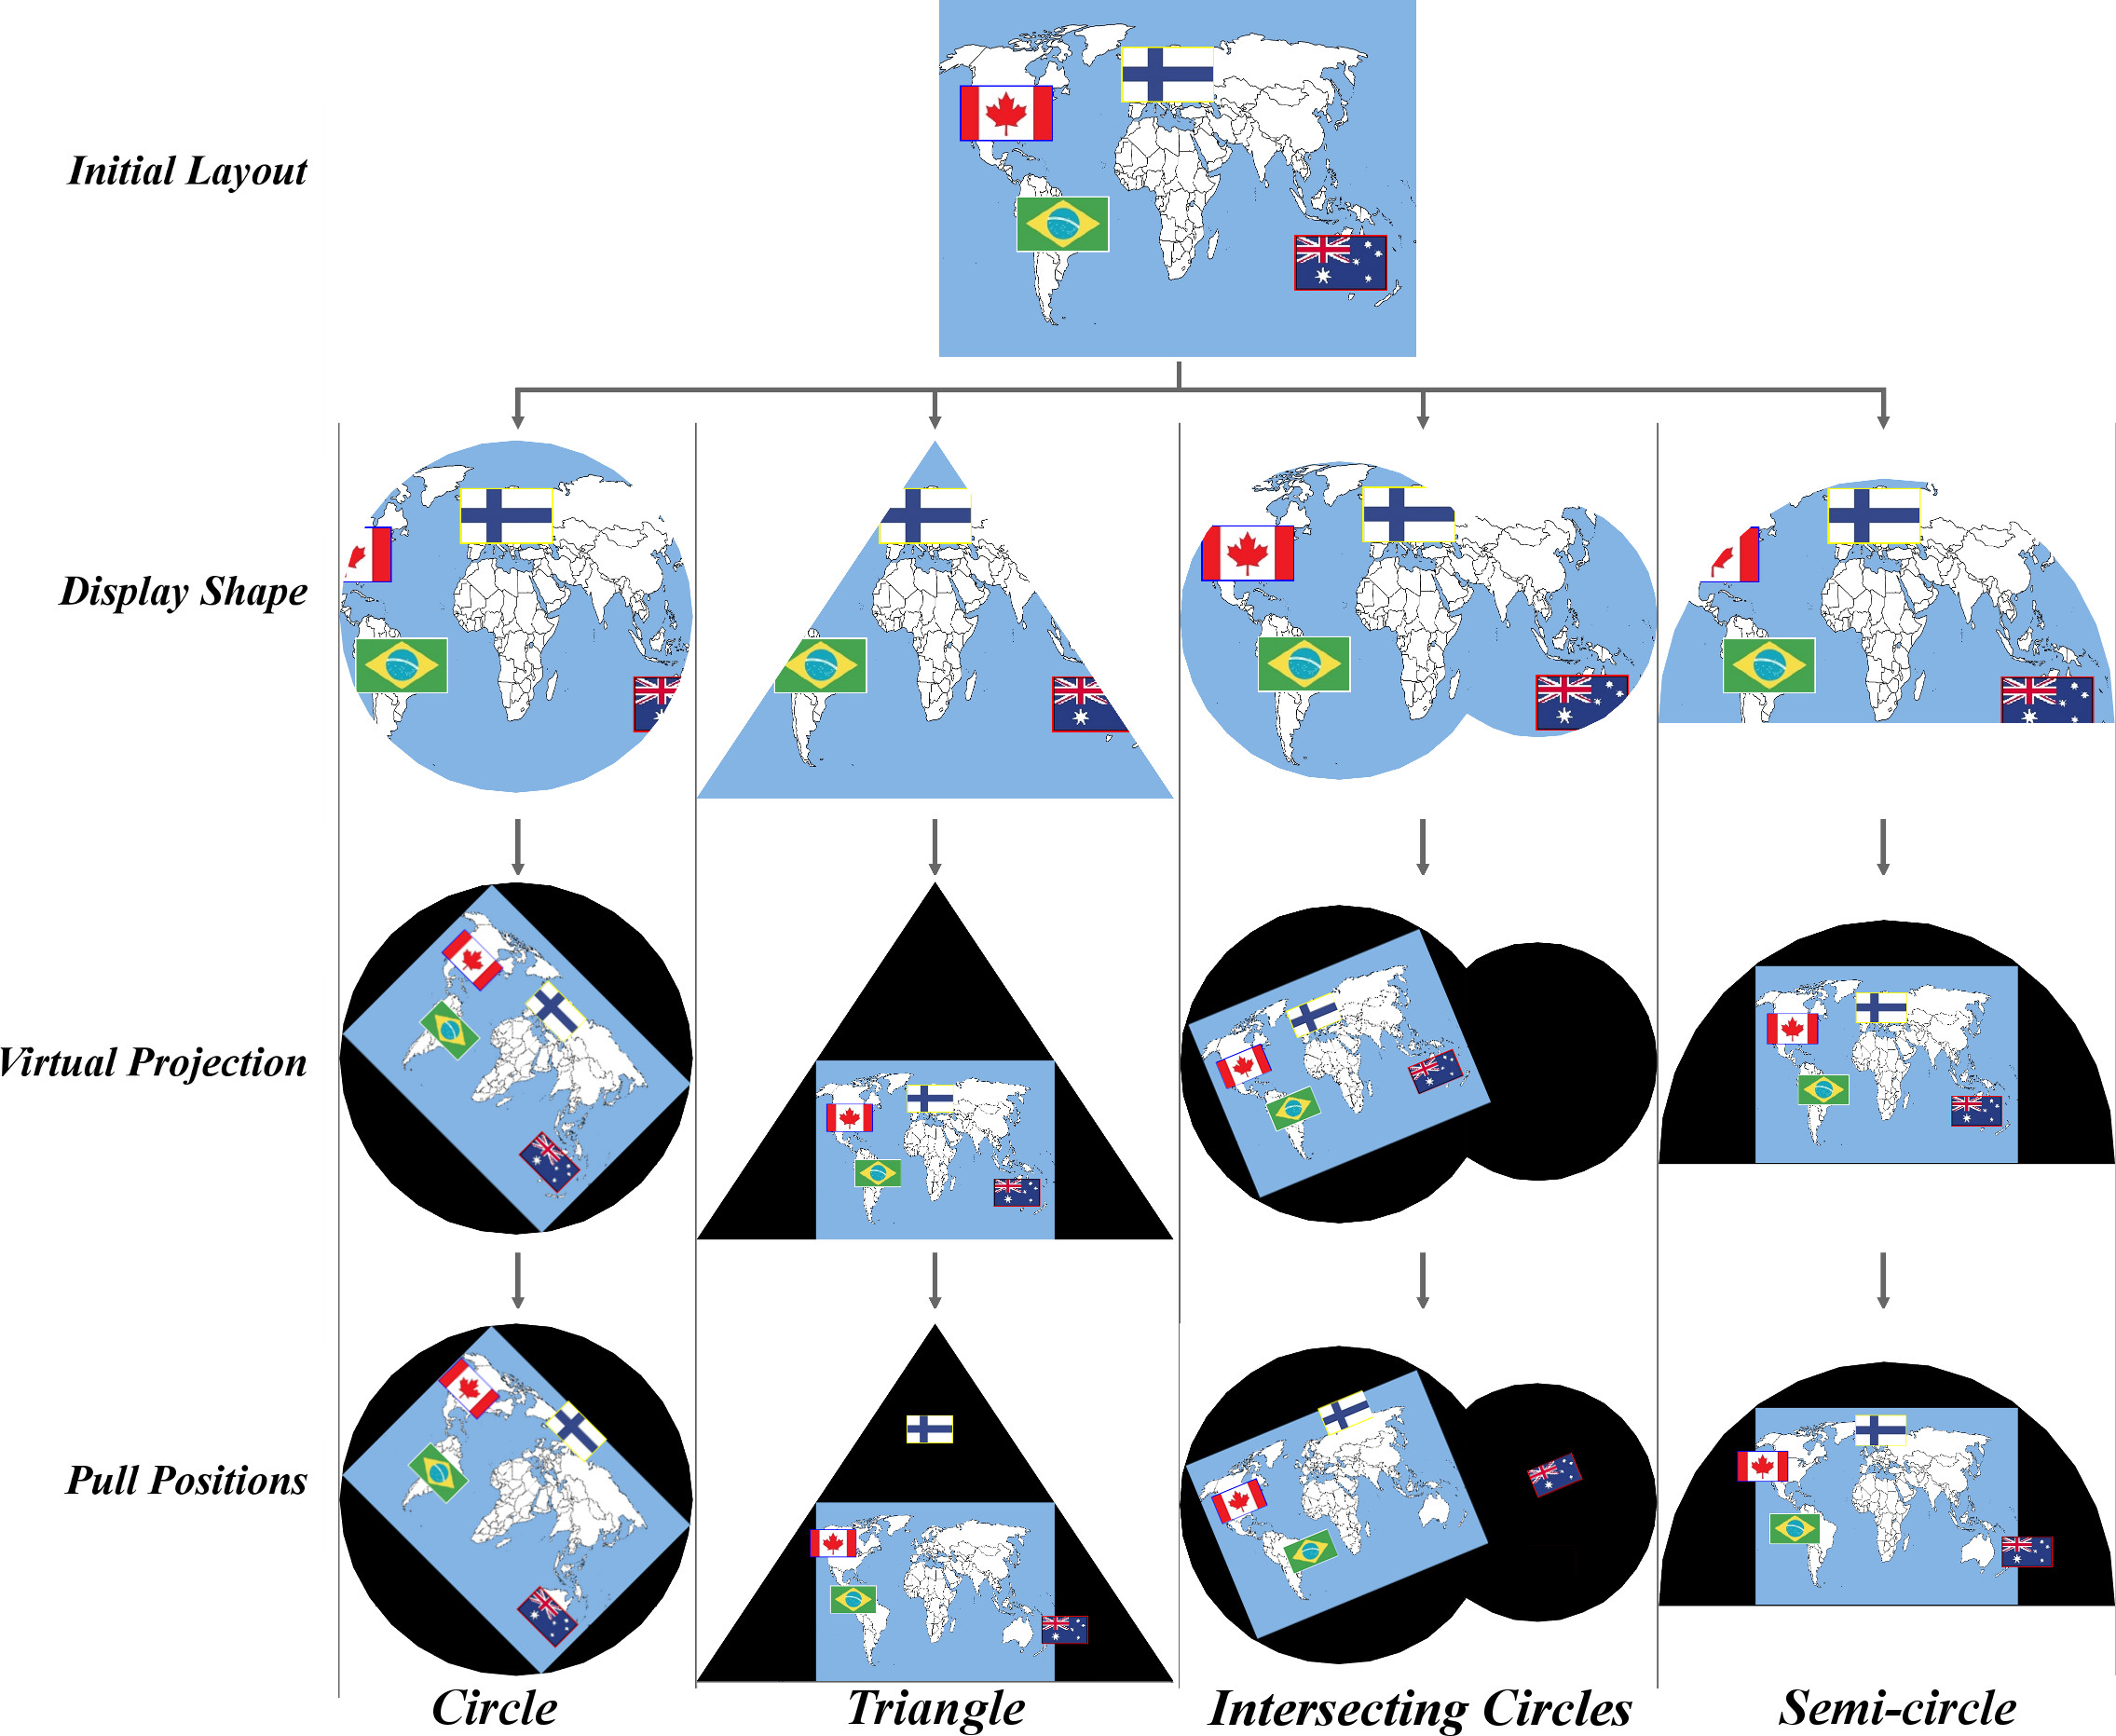
\includegraphics[width=0.9\textwidth]{figures/MapApplication.jpeg}
  \caption{Influence of the implemented technique on {\emph{SynergyNet}}'s {\emph{Simple Map}} application.}
  \label{fig:mapApp}
\end{figure*}

In the map application, the large item displaying the map was made exempt from the influence of the position pulling stage of the technique.

Table~\ref{tab:mapApp} shows that the technique reduced the initial occlusion for all shapes without incurring any additional occlusion from overlapping items or deformation of items throughout its execution.
However, the virtual projection stage did increase the change in scale and the amount of the display shape which went unused.
The pull positions stage of the technique did reduce the amount of the display shape which went unused quite significantly for some shapes but did increase the change in layout.
The change in layout for some of the display shapes was quite significant similar to the grid app implying that the display shape has a large influence on the impact of the technique, not just the content.

Figure~\ref{fig:mapApp} demonstrates the importance of the layout of content items.
Up to the virtual projection stage of the technique, the flag items correctly align with the countries on the map; however, the position pulling stage deforms the layout of the flags in such a way that disengages this alignment.
If it is important for this alignment to be kept then it is best if the flags are made exempt from the position pulling stage of the technique.
As a consequence of this, however, areas of the display will be left unused by the layout.
It therefore becomes a choice developers must make between whether to preserve the layout of content items or to maximise the usage of the display's real estate.
A clear example of this choice can be seen in the technique's influence on the {\emph{Intersecting Circles}} display shape in Figure~\ref{fig:mapApp}.
Without the influence of the position pulling stage of the technique, a large region of the display is left unused by the initial layout, resulting in the {\emph{Display Use \ac{DSDI}}} occurring.
However, with the influence of the position pulling stage of the technique, several of the flag items appear off the map, away from their respective positions, indicating the {\emph{Layout \ac{DSDI}}} has occurred.


%-------------------------------------------------------------------------
\section{Conclusions and Future Work}
\label{sec:conclusion}

Developers must consider the implementation of any proposed method of countering the \acp{DSDI}.
The identification, or creation of, an adequate \ac{DSDI}-minimising technique which allows a particular system to adapt to different display shapes could form part of design guidelines for emerging technologies.
It is important to note that not only the list of \acp{DSDI} for a system should influence the design of a \ac{DSDI}-minimising technique; the need for applications to control the magnitude of a \ac{DSDI}-minimising technique's influence is also important to consider.

The development of the technique presented in Section~\ref{sec:solution} has shown that when designing software for use on differently shaped tabletop displays, the {\emph{Cropping \ac{DSDI}}} must be considered.
In addition to this, secondary \acp{DSDI} which can result from attempts to resolve the initial cropping must also be addressed.
Developers should also consider which \acp{DSDI} their software can tolerate and which must be handled by a \ac{DSDI}-minimising technique.
Choices must be made between whether to preserve the layout of content items or to maximise the display usage.

In the study, all stages of the technique were applied to investigate its impact; in typical usage, an application developer using the framework would have the option to override this for specific content items.
For example, they could apply scale limits to the virtual projection for all content in an application or to individual items.
The ability to choose which stages of the technique affect a content item gives developers control over its influence.
Without this ability there is still a danger of unacceptable \acp{DSDI} occurring in software despite the presence of the implemented technique.
This highlights the importance of any technique intended to minimise the influence of the potential \acp{DSDI} in a system not only to be capable of adapting to different display shapes, but to be also capable of adapting to the needs of the developer. 
This allows developers to make informed, user-centric design and implementation decisions on how content should be displayed.

Developers must consider the limitations of the technique before adopting it.
One such limitation relates to items providing backgrounds.
Depending on what stages of the technique are applied to a background item the result will either be a partially occluded background or blank spaces left where the item is not present due to it being scaled to fit the maximal rectangle.
Both of these outcomes may be undesirable in some scenarios.
There are possible solutions which could be explored however, such as adding an extra step to the technique to apply warping to the background item or context-aware filling of the blank regions of the display.
Another limitation is the assumption of there being no hardware-level attempt to fit the output to the display shape.

It is important to note that although the technique presented in this work is a solution to the \acp{DSDI} of tabletop interfaces, it is not always guaranteed to be the best solution.
It may be possible in many combinations of content and display shapes to find solutions where the impact of the steps taken to avoid \acp{DSDI} is less than the impact of the presented technique.
The solution of less impact may be preferable for developers, as it will allow content to appear more consistent across different displays, allowing for the software to appear more intuitive and familiar for users across devices.
Identifying what solution is best suited for a given situation should be at the centre of any future research involving this topic.
Despite no guarantee that the technique is the optimal solution for a given situation it still is a significant step forward for resolving \acp{DSDI} as it can {\emph{(i)}} always supply an adequate solution to a wide-range of scenarios; {\emph{(ii)}} be automated as part of an implementation as shown in this work; and {\emph{(iii)}} allow developers some control over its execution.

There are a number of reasons why it is important that software becomes display shape independent.
There is now a growing push for software systems to become ubiquitous with the increased availability of natural user interfaces; for a system to become ubiquitous it must fit its environment~\cite{Greenfield2006}.
Being able to change the display shape of a system would aid in achieving this.

\begin{figure}[h!]
 \centering
   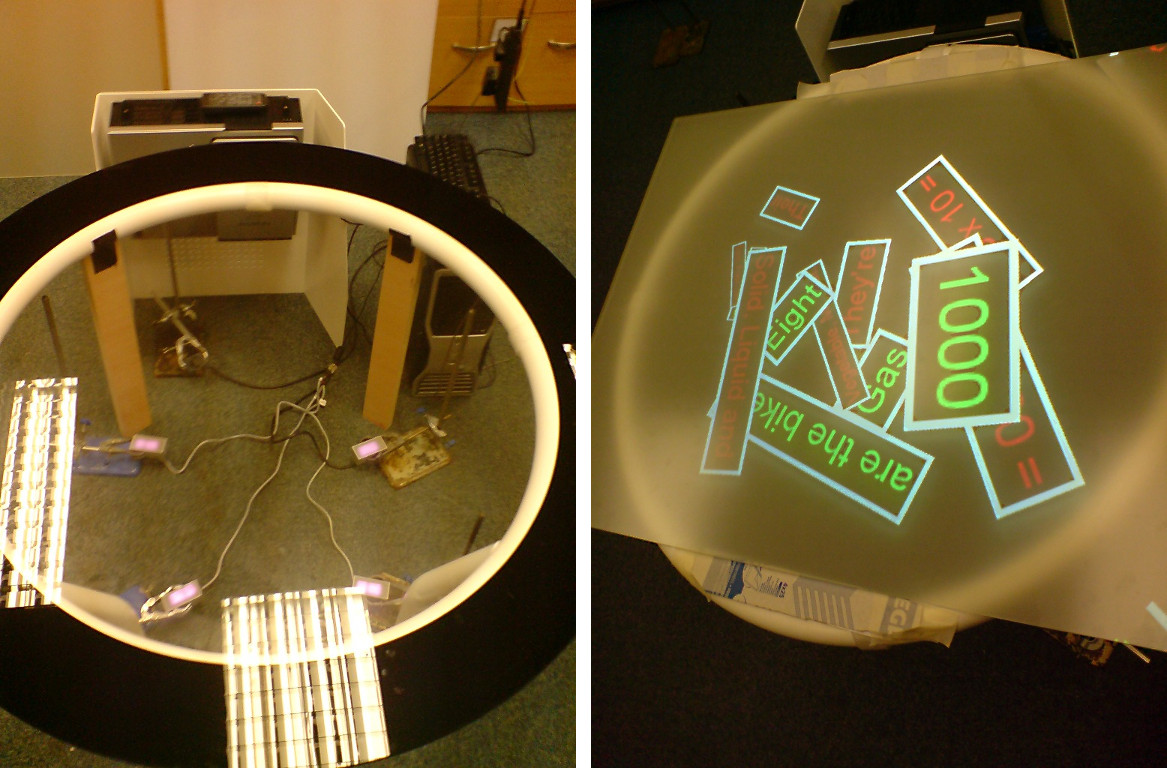
\includegraphics[width=0.45\textwidth]{figures/PrototypeTabletop.jpeg}
   \caption{A prototype of a circular tabletop display.}
   \label{fig:prototypeTabletop}
\end{figure}

The examples of non-rectangular displays discussed in Section~\ref{sec:related} reinforces the need for their support.
In addition to these, many devices brought to market in the recent growth of wearable devices utilise non-rectangular displays, specifically smart watches~\cite{Jung2016}.
Figure~\ref{fig:prototypeTabletop} shows a prototype built by a leasing furniture manufacturer featuring a circular tabletop interface intended for use as an interactive kiosk for public spaces.
The lack of readily available software for the interface's circular display meant that if the tabletop was to be used then bespoke software would need to be commissioned at a significant cost to the manufacturer rather than using any of the readily available off-the-shelf products intended for interactive kiosks.
This highlights the need for making it a simple as possible for software to support different display shapes.

The technique presented in this paper can be adopted by developers to allow their content to fit different display shapes, much like the guidelines presented in the work of Serrano et al.~\cite{Serrano2016,Serrano2017}.
However, while our technique deviates from their guidelines, it provides developers with greater freedom and flexibility.
Without encumbering software developers and content designers with additional restrictions the technique is able to resolve the \acp{DSDI} with minimal input.
This allows for development time to be saved on adding support for different display shapes and also offers more freedom in the design of the content.

Furthermore, the technique outlined in Section~\ref{sec:solution} could also be used beyond tabletop systems.
However, it is possible for the \acp{DSDI} in other systems to vary and differ from those presented in this work~\cite{Serrano2017}. 
For example, attempts to resolve the initial {\emph{Cropping \ac{DSDI}}} may require content items to be rotated.
If a user is viewing the display from a single perspective, such as with a vertical display, then any change in content item's orientation is undesirable.
Information displayed by visual content items, such as text, could appear upside down to the user, making it difficult to read.
However, it is not an issue for systems which allow users to view from multiple perspectives around the display, such as those which utilise horizontal interfaces.
Future work could entail the outlining of \ac{DSDI} for other sets of systems and the production of techniques to minimise their influences.

Further research involving the technique could involve investigating how it functions with more extreme shapes.
Although the shapes used in the implementation of the technique discussed in this study vary greatly and cover a wide range of what is likely to be used as tabletop display shapes, it is possible that shapes that vary from rectangular display in much more extreme ways could be desirable.
Research utilising these extreme shapes could involve finding acceptable limits to place on parts of the technique such as maximum distances to pull content items.

While this work details an implementation of the technique, the next step should be a full user study investigating how the technique works for both real-world developers and end users; for example, a study similar to that carried out by Serrano et al.~\cite{Serrano2017} to review the impact of their proposed guidelines is likely to be a suitable approach.
By instructing developers to utilise the technique when building some software, it should be possible to find out the suitability of the technique in real-world scenarios.
We can then review the impact of the technique in these implementations to find if the results are suitable for end-users.

It is important to note that the scope of this work entailed resolving \acp{DSDI} relating to the layout of visual contents on tabletop interfaces.
Future work has the potential of applying the technique presented to other kinds of interfaces.
This future work would likely focus on additional restrictions the technique would have to take into account, such as the need for a specific orientation with vertical displays.
Future work could also look at expanding the technique to resolve more than just \acp{DSDI} relating to the layout of visual content.
Extra steps or adding limits to the transformations of elements within the technique may help improve usability and readability when applying content to a different display shape.

The technique presented in this paper can be used in various scenarios; one such use of the technique is its implementation into the application layer of a piece of software; this would allow a specific layout of visual content items to be dynamically adapted to different display shapes.
As this implementation of the technique would be customised to the application's specific layout, it would ensure the best results.
However, this does have the drawback that the technique would need to be redefined for every unique application.

Another use for the technique is its implementation into an adaptable and extensible framework.
In a framework-level implementation, the same technique can be
employed by various applications to adapt their visual contents to different display shapes; this is similar to how systems like SUPPLE~\cite{Gajos2004} adapt contents to display parameters.
However, a drawback to this approach is that the technique's implementation may not be suitable for some applications.  
For example, if the technique implementation does not enforce scale limits, the {\emph{Scaling \ac{DSDI}}} may occur.
This may be acceptable for some applications, such as those intended to use content which can still communicate information to the user at any size.
However, it would be unacceptable for other applications, such as those using text.
Therefore, it is important when implementing this technique at a framework level that applications can change how the technique influences them.
The technique's use of higher-level functions, such as the ray firing used in the position pulling stage, make it unsuitable for implementation in lower level software.

The technique could also be implemented as part of a design tool which is used to adapt the layout of visual contents, similar to GUMMY~\cite{Meskens2008}.
Using this implementation, software developers can use the resulting tool to adapt a layout of content items to a specific display shape.
Developers can then make any further changes manually if the tool's automatically generated \ac{DSDI}-minimising technique is not adequate.
Once a developer is satisfied with the software layout they can then specify for its use in their software when the appropriate display shape is present.
This approach has the advantage of allowing developers to check that the layout will be suitable for a specific shape.
However, it does potentially limit the display shapes the system can use to those the developer has input into the tool.

Finally, the technique could be transformed into a set of guidelines for developers to follow when creating software interfaces without the use of a design tool.
The guidelines could also incorporate the decisions to be made concerning the trade-offs in which \acp{DSDI} are minimised.
These guidelines could then be formalised~\cite{Ngo2000}, allowing their application to software to be automated in places.
This would aid with the technique's integration into frameworks and design tools.
With the technique implemented in a tool used to design a wider range of software, its influence can be tested on a wider range of user interfaces with varying complexities in future studies, especially in educational contexts~\cite{McNaughton2017,jg-et-al:2017}.

In summary, the technique presented in this paper is capable of efficiently minimising the effect of the identified \acp{DSDI}, but require trade-offs.
Developers using the technique must decide which \acp{DSDI} could not be tolerated by their software and must adapt the technique according.
Future tabletop software development would benefit greatly from the creation of guidelines to be followed when adapting software to become display shape independent.
The technique produced in this paper, or another similar \ac{DSDI}-minimising technique, should form part of these guidelines.


%============================================%

\CvmAck{
This work was partially funded under the UK's EPSRC/ERSC Teaching and Learning Research Programme (TLRP) {\emph{SynergyNet}} project (RES-139-25-0400).
The authors would also like to thank Professor Liz Burd and Dr Andrew Hatch for their supervision of the primary author's master's degree from which this work originally stems.
The authors would also like to thank the members of the Durham University Technology Enhanced Learning Special Interest Group for supporting the redrafting of this manuscript.
The source code for the technique's implementation presented in this manuscript is available here: \url{https://github.com/synergynet/synergynet2.1}.
}

\bibliographystyle{cvm}

{\normalsize  \bibliography{DSDI-CVM}}

\Author{bio-james}{James McNaughton}
{is a researcher at Durham University (UK) whose research interests include HCI, natural user interfaces and augmented reality.
His current work involves investigating the use of emerging interaction technologies in classroom environments.}

\Author{bio-tom}{Tom Crick}
{is Professor of Digital Education \& Policy at Swansea University (UK).
His research interests are interdisciplinary, data-driven and computationally-intensive, including data science, intelligent systems, software sustainability, public service innovation and STEM education.}

\Author{bio-shamus}{Shamus Smith}
{is a Lecturer in Computer Science at the University of Newcastle (Australia).
His current research interests include touch-based technologies, mobile technology for augmented reality and the reuse of gaming technology.} 

\end{document}
